\documentclass[12pt,letterpaper,twoside]{report}

% ============================================
% PAQUETES ESENCIALES
% ============================================
\usepackage[utf8]{inputenc}
\usepackage[spanish,es-tabla]{babel}
\usepackage[T1]{fontenc}
\usepackage{lmodern}
\usepackage{amsmath,amssymb,amsthm}
\usepackage{mathtools}
\usepackage{graphicx}
\usepackage{booktabs}
\usepackage{longtable}
\usepackage{multirow}
\usepackage{array}
\usepackage{tabularx}
\usepackage[table,xcdraw]{xcolor}
\usepackage{float}
\usepackage{subcaption}
\usepackage{geometry}
\usepackage{fancyhdr}
\usepackage{hyperref}
\usepackage{cleveref}
\usepackage{enumitem}
\usepackage{algorithm}
\usepackage{algpseudocode}
\usepackage{listings}
\usepackage{xcolor}
\usepackage{tcolorbox}
\usepackage{tikz}
\usetikzlibrary{shapes,arrows,positioning,calc}

% ============================================
% CONFIGURACIÓN DE PÁGINA
% ============================================
\geometry{
    letterpaper,
    left=3cm,
    right=2.5cm,
    top=2.5cm,
    bottom=2.5cm,
    headheight=15pt
}

\pagestyle{fancy}
\fancyhf{}
\fancyhead[LE,RO]{\thepage}
\fancyhead[LO]{\nouppercase{\rightmark}}
\fancyhead[RE]{\nouppercase{\leftmark}}

% ============================================
% CONFIGURACIÓN DE HYPERREF
% ============================================
\hypersetup{
    colorlinks=true,
    linkcolor=blue,
    filecolor=magenta,      
    urlcolor=cyan,
    citecolor=green,
    pdftitle={Informe Técnico Pipeline Bioestadístico},
    pdfauthor={Luis Ángel Martínez},
}

% ============================================
% CONFIGURACIÓN DE LISTINGS (CÓDIGO)
% ============================================
\lstdefinestyle{pythonstyle}{
    language=Python,
    basicstyle=\ttfamily\footnotesize,
    keywordstyle=\color{blue}\bfseries,
    commentstyle=\color{gray}\itshape,
    stringstyle=\color{red},
    numbers=left,
    numberstyle=\tiny\color{gray},
    stepnumber=1,
    numbersep=10pt,
    backgroundcolor=\color{white},
    showspaces=false,
    showstringspaces=false,
    showtabs=false,
    frame=single,
    rulecolor=\color{black},
    tabsize=4,
    captionpos=b,
    breaklines=true,
    breakatwhitespace=false,
    escapeinside={\%*}{*)},
    xleftmargin=2em,
    framexleftmargin=1.5em
}

\lstset{style=pythonstyle}

% ============================================
% ENTORNOS PERSONALIZADOS
% ============================================
\newtcolorbox{hipotesisbox}[1][]{
    colback=blue!5!white,
    colframe=blue!75!black,
    title={\textbf{Paso 1: Planteamiento de Hipótesis}},
    fonttitle=\bfseries,
    #1
}

\newtcolorbox{estadisticobox}[1][]{
    colback=green!5!white,
    colframe=green!75!black,
    title={\textbf{Paso 2: Selección del Estadístico/Método}},
    fonttitle=\bfseries,
    #1
}

\newtcolorbox{reglabox}[1][]{
    colback=orange!5!white,
    colframe=orange!75!black,
    title={\textbf{Paso 3: Regla de Decisión}},
    fonttitle=\bfseries,
    #1
}

\newtcolorbox{calculobox}[1][]{
    colback=purple!5!white,
    colframe=purple!75!black,
    title={\textbf{Paso 4: Cálculos}},
    fonttitle=\bfseries,
    #1
}

\newtcolorbox{decisionbox}[1][]{
    colback=red!5!white,
    colframe=red!75!black,
    title={\textbf{Paso 5: Decisión Estadística}},
    fonttitle=\bfseries,
    #1
}

\newtcolorbox{conclusionbox}[1][]{
    colback=cyan!5!white,
    colframe=cyan!75!black,
    title={\textbf{Paso 6: Conclusión}},
    fonttitle=\bfseries,
    #1
}

% ============================================
% COMANDOS PERSONALIZADOS
% ============================================
\newcommand{\vect}[1]{\boldsymbol{#1}}
\newcommand{\mat}[1]{\mathbf{#1}}
\newcommand{\R}{\mathbb{R}}
\newcommand{\N}{\mathbb{N}}
\newcommand{\E}{\mathbb{E}}
\newcommand{\Var}{\mathrm{Var}}
\newcommand{\Cov}{\mathrm{Cov}}

% ============================================
% INFORMACIÓN DEL DOCUMENTO
% ============================================
\title{
    \vspace{-2cm}
    \Huge\textbf{Informe Técnico Completo} \\[0.5cm]
    \LARGE Pipeline Bioestadístico para la Clasificación de\\
    Sedentarismo mediante Lógica Difusa y Clustering\\[0.3cm]
    \Large Perspectiva Bioestadística, Clínica y Computacional
}
\author{
    \Large Luis Ángel Martínez\\[0.2cm]
    \large Universidad Autónoma de Chihuahua\\
    \large Facultad de Medicina y Ciencias Biomédicas\\[0.2cm]
    \normalsize Programa de Maestría en Ciencias de la Salud
}
\date{\today}

% ============================================
% INICIO DEL DOCUMENTO
% ============================================
\begin{document}

\maketitle

\begin{abstract}
\noindent
El presente informe técnico documenta de manera exhaustiva el pipeline bioestadístico desarrollado para la clasificación objetiva del sedentarismo semanal utilizando datos biométricos de dispositivos wearables (Apple Watch). Este proyecto representa un estudio longitudinal con $N=10$ participantes (5M/5H) que generaron 1,337 semanas válidas de datos continuos.

El pipeline integra tres perspectivas complementarias: \textbf{bioestadística} (modelado probabilístico robusto, reducción dimensional, clustering, validación), \textbf{clínica} (normalización antropométrica, interpretación fisiológica de variables derivadas, relevancia para ciencias del ejercicio), y \textbf{computacional} (arquitectura modular en Python, estrategias de imputación jerárquica, optimización de hiperparámetros).

Metodológicamente, el estudio pivotó de un enfoque supervisado inicial (predicción de Calidad de Vida mediante Redes Neuronales Artificiales, invalidado empíricamente) a un paradigma \textit{data-driven} dual: (1) descubrimiento de patrones mediante clustering no supervisado (K-Means, $K=2$, Silhouette$=0.232$), empleado como \textbf{Verdad Operativa (GO)}, y (2) construcción de un Sistema de Inferencia Difusa Mamdani interpretable con 5 reglas expertas, validado contra la GO con $F1=0.840$, Recall$=0.976$, MCC$=0.294$.

Cada fase del pipeline se presenta bajo el marco riguroso de los \textbf{6 pasos del análisis estadístico}: planteamiento de hipótesis, selección del estadístico, regla de decisión, cálculos, decisión estadística y conclusión. Se incluyen ecuaciones matemáticas formales, pseudocódigo, referencias a figuras y tablas, y una justificación detallada de la decisión metodológica de \textit{no} emplear un split Train/Test 80/20, reemplazado por validación cruzada Leave-One-User-Out (LOUO) y análisis de sensibilidad.

\textbf{Palabras clave}: Sedentarismo, Wearables, Apple Watch, Lógica Difusa, Clustering, K-Means, Imputación Jerárquica, Ingeniería de Características, Validación Cruzada, Python.
\end{abstract}

\tableofcontents

% ============================================
% CAPÍTULO 1: PLANTEAMIENTO DEL PROBLEMA
% ============================================
\chapter{Planteamiento del Problema e Hipótesis Inicial}

\section{Contexto Epidemiológico y Clínico}

El comportamiento sedentario (CS), definido por la Organización Mundial de la Salud como cualquier actividad con gasto energético $\leq 1.5$ METs en posición sentada o reclinada durante horas de vigilia, constituye un factor de riesgo independiente para enfermedades crónicas no transmisibles (ECNT), incluyendo obesidad, diabetes tipo 2, enfermedad cardiovascular y ciertos tipos de cáncer \cite{who2020}.

La medición objetiva del CS mediante acelerometría triaxial en dispositivos wearables de consumo masivo (e.g., Apple Watch, Fitbit, Garmin) ha revolucionado la epidemiología del comportamiento, permitiendo cuantificar patrones de actividad física en condiciones de ``vida libre'' con alta resolución temporal ($\geq 1$ Hz) y sin el sesgo de auto-reporte característico de cuestionarios.

\section{Hipótesis Inicial y Objetivo Primario}

\begin{hipotesisbox}
\textbf{Hipótesis H$_0$ (inicial, posteriormente rechazada):}

Existe una relación inversa, lineal y medible entre el comportamiento sedentario objetivo (CS\_obj), cuantificado mediante métricas derivadas de acelerometría y fotopletismografía (PPG) del Apple Watch, y la percepción subjetiva de Calidad de Vida Relacionada con la Salud (CVRS), evaluada mediante el cuestionario SF-36.

Formalmente:
\begin{equation}
\text{CVRS}_{SF36} = f(\text{CS}_{\text{obj}}) + \epsilon, \quad \epsilon \sim \mathcal{N}(0, \sigma^2)
\end{equation}

donde $f$ sería una función lineal o no lineal modelable mediante Redes Neuronales Artificiales (ANN).
\end{hipotesisbox}

\subsection{Objetivo Primario (Fase Inicial)}

Desarrollar un modelo predictivo (ANN) capaz de cuantificar la CVRS a partir de métricas biométricas continuas, con $R^2 \geq 0.70$ y MAE $\leq 10$ puntos en escala SF-36.

\section{Marco de los 6 Pasos: Planteamiento}

\begin{estadisticobox}
\textbf{Selección del método:}

Se propuso inicialmente un análisis correlacional (Pearson/Spearman) seguido de modelado supervisado mediante ANN (arquitectura feedforward, activación ReLU, optimizador Adam).
\end{estadisticobox}

\begin{reglabox}
\textbf{Regla de decisión:}

Si $|r| \geq 0.60$ (correlación fuerte) y el modelo ANN alcanza $R^2 \geq 0.70$ en validación cruzada 5-fold, se aceptará la hipótesis de relación cuantificable.
\end{reglabox}

\begin{decisionbox}
\textbf{Decisión preliminar:}

Se decidió proceder con un diseño longitudinal que recolectaría datos biométricos continuos (Apple Watch) y evaluaciones periódicas del SF-36 para probar esta correlación.
\end{decisionbox}

\begin{conclusionbox}
\textbf{Conclusión del planteamiento:}

Existía suficiente justificación teórica (revisión de literatura: correlaciones reportadas entre actividad física y CVRS en el rango $r=0.30-0.50$) para explorar esta vía, aunque con la precaución de que la relación podría ser más compleja de lo anticipado.
\end{conclusionbox}

% ============================================
% CAPÍTULO 2: SELECCIÓN DE DISPOSITIVO Y POBLACIÓN
% ============================================
\chapter{Selección del Dispositivo Wearable y Diseño de la Cohorte}

\section{Evaluación de Dispositivos Wearables}

\subsection{Criterios de Selección}

\begin{hipotesisbox}
\textbf{Problema/Hipótesis:}

Necesitábamos un dispositivo wearable que cumpliera simultáneamente:
\begin{itemize}[noitemsep]
    \item Alta penetración de mercado (facilitar reclutamiento BYOD)
    \item Sensores validados: acelerómetro 3-ejes ($\geq 50$ Hz), PPG para FC/VFC
    \item Plataforma de exportación de datos crudos o agregados
    \item Consistencia inter-versión (minimizar heterogeneidad instrumental)
\end{itemize}

Hipótesis: El Apple Watch, por su ecosistema cerrado y validaciones previas en literatura (Stahl et al., 2016; Shcherbina et al., 2017), sería la opción preferente.
\end{hipotesisbox}

\subsection{Análisis Comparativo}

\begin{table}[H]
\centering
\caption{Matriz de Decisión: Comparación de Dispositivos Wearables}
\label{tab:wearables_comparison}
\begin{tabular}{@{}lcccc@{}}
\toprule
\textbf{Criterio} & \textbf{Apple Watch} & \textbf{Fitbit} & \textbf{Garmin} & \textbf{Mi Band} \\
\midrule
Penetración México & Alta & Media & Media-Baja & Alta \\
Sensores validados & Sí & Sí & Sí & Parcial \\
Exportación datos & HealthKit (XML) & API limitada & Garmin Connect & Propietaria \\
Consistencia HW & Alta & Media & Alta & Baja \\
Costo promedio (USD) & 300-800 & 100-300 & 250-700 & 30-50 \\
\textbf{Score ponderado} & \textbf{9.2} & 7.5 & 7.8 & 5.1 \\
\bottomrule
\end{tabular}
\end{table}

\begin{estadisticobox}
\textbf{Método de evaluación:}

Matriz de decisión multicriterio con pesos asignados según importancia para el estudio:
\begin{itemize}[noitemsep]
    \item Validez de sensores: 35\%
    \item Exportabilidad de datos: 30\%
    \item Consistencia: 20\%
    \item Penetración: 15\%
\end{itemize}
\end{estadisticobox}

\begin{decisionbox}
\textbf{Decisión:}

Se seleccionó el \textbf{Apple Watch} (Series 3 o superior) como dispositivo estándar del estudio, adoptando un enfoque \textit{Bring Your Own Device} (BYOD) para maximizar adherencia y minimizar el efecto Hawthorne.
\end{decisionbox}

\section{Diseño de la Cohorte}

\subsection{Tamaño Muestral y Justificación}

\begin{hipotesisbox}
\textbf{Planteamiento:}

Dada la naturaleza longitudinal del estudio (objetivo: capturar variabilidad intra-sujeto durante $\geq 12$ semanas), el tamaño muestral $N$ se justificó por:

\begin{equation}
n_{\text{observaciones}} = N_{\text{sujetos}} \times T_{\text{semanas}} \geq 1000
\end{equation}

Con $N=10$ y $T \approx 130$ semanas (promedio), se alcanzarían $\approx 1300$ observaciones semanales, suficiente para:
\begin{itemize}[noitemsep]
    \item Modelado de clustering con $n/K \geq 500$ por grupo ($K=2$)
    \item Optimización de hiperparámetros del sistema difuso
    \item Validación cruzada Leave-One-Subject-Out
\end{itemize}
\end{hipotesisbox}

\subsection{Criterios de Inclusión/Exclusión}

\begin{table}[H]
\centering
\caption{Criterios de Elegibilidad de Participantes}
\label{tab:eligibility}
\begin{tabular}{@{}p{4cm}p{5cm}p{5cm}@{}}
\toprule
\textbf{Criterio} & \textbf{Inclusión} & \textbf{Exclusión} \\
\midrule
Edad & 18-65 años & $<18$ o $>65$ años \\
Dispositivo & Propietario Apple Watch Series $\geq 3$ & Sin dispositivo o Series $<3$ \\
Uso previo & $\geq 6$ meses continuos & $<6$ meses (sesgo familiarización) \\
Estado de salud & Ambulatorio, sin limitaciones & Limitaciones severas movilidad \\
Consentimiento & Informado por escrito & Negativa o retiro \\
Datos exportables & $\geq 80\%$ días con datos & $<80\%$ (adherencia insuficiente) \\
\bottomrule
\end{tabular}
\end{table}

\begin{calculobox}
\textbf{Cálculos de factibilidad:}

Se convocó a 15 candidatos, de los cuales:
\begin{itemize}[noitemsep]
    \item 12 cumplieron criterios de inclusión
    \item 10 completaron el protocolo (2 abandonos por causas no relacionadas)
    \item Distribución final: 5 hombres, 5 mujeres
    \item Edad: $\bar{x}=32.4$ años, $s=8.7$ años
    \item IMC: $\bar{x}=26.1$ kg/m$^2$, $s=4.2$ kg/m$^2$
\end{itemize}
\end{calculobox}

\begin{conclusionbox}
\textbf{Conclusión metodológica:}

Aunque no representativa poblacionalmente (muestra de conveniencia), la cohorte de $N=10$ permite un análisis longitudinal profundo con potencia estadística adecuada para el descubrimiento de patrones intra-sujeto y validación de sistemas expertos interpretativos (objetivo secundario tras el pivote metodológico).
\end{conclusionbox}

% ============================================
% CAPÍTULO 3: CONVOCATORIA Y PREPROCESAMIENTO
% ============================================
\chapter{Protocolo de Convocatoria, Recepción y Preprocesamiento de Datos}

\section{Protocolo de Recolección de Datos}

\subsection{Diseño del Protocolo}

\begin{hipotesisbox}
\textbf{Planteamiento:}

Para garantizar la integridad, trazabilidad y ética de los datos biométricos sensibles, se diseñó un protocolo estandarizado que incluye:
\begin{enumerate}[noitemsep]
    \item Consentimiento informado (aprobación comité ética institucional)
    \item Instrucciones de exportación (HealthKit $\to$ archivo \texttt{export.zip})
    \item Aplicación del cuestionario SF-36 (versión mexicana validada)
    \item Anonimización inmediata (códigos: u1, u2, ..., u10)
    \item Almacenamiento seguro (servidor institucional, encriptación AES-256)
\end{enumerate}
\end{hipotesisbox}

\subsection{Estructura de Datos Crudos}

Los datos exportados de Apple Health siguen el esquema XML:

\begin{lstlisting}[language=XML, caption={Estructura XML de Apple Health Export}]
<HealthData>
  <Record type="HKQuantityTypeIdentifierStepCount"
          sourceName="Apple Watch de Luis"
          value="1245"
          unit="count"
          startDate="2023-10-22 08:15:00"
          endDate="2023-10-22 08:16:00"/>
  ...
</HealthData>
\end{lstlisting}

\section{Pipeline de Preprocesamiento}

\subsection{Conversión XML $\to$ CSV}

\begin{estadisticobox}
\textbf{Método:}

Parseo XML mediante \texttt{ElementTree} (Python), con transformaciones:
\begin{itemize}[noitemsep]
    \item Filtrado por \texttt{sourceName} (solo datos Apple Watch, excluir iPhone)
    \item Conversión de timestamps a zona horaria local (UTC-6, Chihuahua)
    \item Agregación a nivel diario (suma/media según métrica)
\end{itemize}
\end{estadisticobox}

\begin{algorithm}[H]
\caption{Preprocesamiento XML a CSV Diario}
\label{alg:xml_to_csv}
\begin{algorithmic}[1]
\State \textbf{Input:} \texttt{export.zip} por participante
\State \textbf{Output:} \texttt{DB\_u\{id\}.csv} con columnas [fecha, pasos, calorias, fc\_reposo, hrv\_sdnn, ...]
\State
\Procedure{ParseXML}{xml\_file, user\_id}
    \State tree $\gets$ parse(xml\_file)
    \State records $\gets$ tree.findall("Record")
    \State df $\gets$ empty\_dataframe()
    \For{record \textbf{in} records}
        \If{record.sourceName \textbf{contains} "Apple Watch"}
            \State type $\gets$ record.type
            \State value $\gets$ record.value
            \State date $\gets$ record.startDate.date()
            \State df.append([date, type, value])
        \EndIf
    \EndFor
    \State df\_pivot $\gets$ df.pivot(index=date, columns=type, values=value)
    \State df\_pivot.to\_csv(f"DB\_u\{user\_id\}.csv")
\EndProcedure
\end{algorithmic}
\end{algorithm}

\begin{calculobox}
\textbf{Cálculos de agregación:}

Para cada usuario y día:
\begin{align}
\text{Pasos}_{\text{día}} &= \sum_{t=0}^{23:59} \text{StepCount}(t) \\
\text{FC}_{\text{reposo}} &= \text{min}\{\text{HeartRate}(t) : t \in [02:00, 05:00]\} \\
\text{HRV\_SDNN}_{\text{día}} &= \text{mean}\{\text{SDNN}(t) : t \in [00:00, 23:59]\}
\end{align}
\end{calculobox}

\subsection{Auditoría de Calidad de Datos}

\begin{table}[H]
\centering
\caption{Métricas de Completitud por Usuario (Fase Pre-Imputación)}
\label{tab:data_quality_raw}
\begin{tabular}{@{}lrrrrr@{}}
\toprule
\textbf{Usuario} & \textbf{Días totales} & \textbf{Días válidos} & \textbf{Completitud (\%)} & \textbf{Missing FC (\%)} & \textbf{Missing HRV (\%)} \\
\midrule
u1  & 900 & 852 & 94.7 & 8.2 & 15.3 \\
u2  & 850 & 801 & 94.2 & 9.1 & 17.8 \\
u3  & 920 & 884 & 96.1 & 5.4 & 12.1 \\
... & ... & ... & ... & ... & ... \\
u10 & 880 & 831 & 94.4 & 7.8 & 14.9 \\
\midrule
\textbf{Media} & \textbf{885} & \textbf{838} & \textbf{94.7} & \textbf{7.6} & \textbf{14.8} \\
\bottomrule
\end{tabular}
\end{table}

\begin{decisionbox}
\textbf{Decisión:}

La completitud general $>94\%$ es aceptable para estudios observacionales de vida libre. Las variables cardiovasculares (FC, HRV) presentan mayor tasa de missingness (mecanismo: quitarse el reloj durante sueño/carga), requiriendo estrategia de imputación robusta (Capítulo 6).
\end{decisionbox}

% ============================================
% CAPÍTULO 4: ANÁLISIS EXPLORATORIO INICIAL
% ============================================
\chapter{Análisis Exploratorio de Datos (EDA) y Validación del SF-36}

\section{Caracterización de Variables Biométricas}

\subsection{Tipología y Distribuciones}

\begin{hipotesisbox}
\textbf{Hipótesis:}

Se esperaba que las variables biométricas diarias presentaran:
\begin{itemize}[noitemsep]
    \item Distribuciones asimétricas (pasos, minutos ejercicio: asimetría positiva)
    \item Alta variabilidad día-a-día (CV $> 50\%$)
    \item No-normalidad (rechazo de Shapiro-Wilk con $p<0.05$)
\end{itemize}
\end{hipotesisbox}

\begin{estadisticobox}
\textbf{Métodos aplicados:}

\begin{itemize}[noitemsep]
    \item Estadísticos descriptivos robustos: mediana, IQR, MAD
    \item Pruebas de normalidad: Shapiro-Wilk (si $n<5000$), Kolmogorov-Smirnov (si $n \geq 5000$)
    \item Visualización: histogramas, Q-Q plots, boxplots por usuario
\end{itemize}
\end{estadisticobox}

\begin{table}[H]
\centering
\caption{Estadísticos Descriptivos de Variables Clave (Nivel Diario, $n=8,380$ días)}
\label{tab:descriptive_daily}
\resizebox{\textwidth}{!}{%
\begin{tabular}{@{}lrrrrrrc@{}}
\toprule
\textbf{Variable} & \textbf{Media} & \textbf{DE} & \textbf{Mediana} & \textbf{IQR} & \textbf{Min} & \textbf{Max} & \textbf{SW $p$-valor} \\
\midrule
Pasos             & 6,842 & 4,231 & 6,120 & 4,890 & 0    & 28,450 & $<0.001$ \\
Calorías activas  & 385   & 287   & 342   & 298   & 0    & 1,892  & $<0.001$ \\
FC reposo (lpm)   & 58.3  & 8.7   & 57.0  & 10.0  & 42   & 92     & $0.014$ \\
HRV SDNN (ms)     & 52.1  & 18.4  & 48.5  & 22.0  & 15   & 128    & $<0.001$ \\
FC caminar (lpm)  & 95.8  & 12.3  & 94.0  & 15.0  & 65   & 145    & $0.082$ \\
Min sedentarios   & 678   & 142   & 702   & 185   & 120  & 1,320  & $<0.001$ \\
\bottomrule
\end{tabular}%
}
\end{table}

\begin{decisionbox}
\textbf{Decisión estadística:}

Se rechaza la normalidad para todas las variables excepto FC\_caminar ($p=0.082$). Consecuencia: uso obligatorio de métodos no paramétricos o robustos (medianas, bootstrapping, Mann-Whitney U) en análisis posteriores.
\end{decisionbox}

\subsection{Gráficos Exploratorios}

\textbf{Gráficos exploratorios generados (disponibles en \texttt{analisis\_u/}):}

\textit{Nota: Figuras de histogramas, Q-Q plots y boxplots por usuario disponibles en el directorio \texttt{figuras/} para referencia detallada.}

\section{Validación Psicométrica del SF-36}

\subsection{Estructura del Cuestionario}

El SF-36 evalúa 8 dimensiones de CVRS mediante 36 ítems:
\begin{itemize}[noitemsep]
    \item Función Física (FF)
    \item Rol Físico (RF)
    \item Dolor Corporal (DC)
    \item Salud General (SG)
    \item Vitalidad (VT)
    \item Función Social (FS)
    \item Rol Emocional (RE)
    \item Salud Mental (SM)
\end{itemize}

\begin{estadisticobox}
\textbf{Métrica de fiabilidad:}

Alfa de Cronbach por dimensión, criterio $\alpha \geq 0.70$ (aceptable).

\begin{equation}
\alpha = \frac{K}{K-1} \left( 1 - \frac{\sum_{i=1}^{K} \sigma^2_i}{\sigma^2_{\text{total}}} \right)
\end{equation}

donde $K$ = número de ítems, $\sigma^2_i$ = varianza del ítem $i$.
\end{estadisticobox}

\begin{table}[H]
\centering
\caption{Fiabilidad del SF-36 en la Cohorte ($N=10$)}
\label{tab:sf36_reliability}
\begin{tabular}{@{}lrrc@{}}
\toprule
\textbf{Dimensión SF-36} & \textbf{$\alpha$ Cronbach} & \textbf{Varianza} & \textbf{Decisión} \\
\midrule
Función Física    & 0.82 & 145.3 & \textcolor{green}{Aceptable} \\
Rol Físico        & 0.51 & 0.0   & \textcolor{red}{Rechazada (var=0)} \\
Dolor Corporal    & 0.78 & 98.7  & \textcolor{green}{Aceptable} \\
Salud General     & 0.73 & 112.4 & \textcolor{green}{Aceptable} \\
Vitalidad         & 0.64 & 87.2  & \textcolor{orange}{Marginal} \\
Función Social    & 0.71 & 102.1 & \textcolor{green}{Aceptable} \\
Rol Emocional     & 0.76 & 118.5 & \textcolor{green}{Aceptable} \\
Salud Mental      & 0.80 & 134.2 & \textcolor{green}{Aceptable} \\
\bottomrule
\end{tabular}
\end{table}

\begin{decisionbox}
\textbf{Decisión crítica:}

La dimensión \textbf{Rol Físico} presenta varianza nula (todos los participantes reportaron el mismo valor, efecto techo/suelo), invalidando su uso. Vitalidad ($\alpha=0.64$) está por debajo del umbral.

\textbf{Consecuencia}: Estos problemas psicométricos, sumados a correlaciones débiles con biométricos (siguiente sección), motivaron el rechazo de la hipótesis inicial y el pivote metodológico.
\end{decisionbox}

\begin{conclusionbox}
\textbf{Conclusión EDA:}

\begin{enumerate}[noitemsep]
    \item Los datos biométricos son ruidosos y no-normales, requiriendo métodos robustos.
    \item El SF-36 presenta limitaciones en esta cohorte específica (tamaño, homogeneidad).
    \item La alta variabilidad diaria (CV $> 100\%$ en ejercicio) justifica agregación temporal (semanal) para capturar patrones estables.
\end{enumerate}
\end{conclusionbox}

% ============================================
% CAPÍTULO 5: PIVOTE METODOLÓGICO
% ============================================
\chapter{Pivote Metodológico: Del Enfoque Supervisado al Data-Driven}

\section{Análisis de Correlación SF-36 vs Biométricos}

\subsection{Hipótesis y Pruebas Iniciales}

\begin{hipotesisbox}
\textbf{Hipótesis H$_1$ a probar:}

Las métricas biométricas agregadas (media de 4 semanas) correlacionan significativamente ($|r| \geq 0.60$, $p<0.01$) con los puntajes de CVRS del SF-36.
\end{hipotesisbox}

\begin{estadisticobox}
\textbf{Métodos:}

\begin{itemize}[noitemsep]
    \item Correlación de Spearman (datos no-normales)
    \item Corrección Bonferroni para comparaciones múltiples ($\alpha^* = 0.05 / 32 = 0.0016$)
    \item Scatter plots con líneas de regresión LOWESS
\end{itemize}
\end{estadisticobox}

\begin{table}[H]
\centering
\caption{Matriz de Correlación: Biométricos Agregados vs SF-36 ($N=10$)}
\label{tab:correlation_sf36}
\resizebox{\textwidth}{!}{%
\begin{tabular}{@{}lrrrrrrrr@{}}
\toprule
 & \textbf{FF} & \textbf{RF} & \textbf{DC} & \textbf{SG} & \textbf{VT} & \textbf{FS} & \textbf{RE} & \textbf{SM} \\
\midrule
Pasos promedio        & 0.32 & --- & 0.18 & 0.41 & -0.05 & 0.27 & 0.14 & 0.09 \\
Calorías promedio     & 0.38 & --- & 0.22 & 0.45 & -0.12 & 0.31 & 0.19 & 0.13 \\
FC reposo promedio    & -0.21 & --- & -0.14 & -0.28 & 0.08 & -0.18 & -0.11 & -0.06 \\
HRV SDNN promedio     & 0.15 & --- & 0.09 & 0.24 & 0.31 & 0.12 & 0.08 & 0.19 \\
Min sedentarios       & -0.29 & --- & -0.16 & -0.35 & -0.18 & -0.24 & -0.13 & -0.11 \\
\bottomrule
\multicolumn{9}{l}{\footnotesize \textit{Nota}: RF excluido por varianza nula. Ninguna correlación alcanza $|r| \geq 0.60$ ni $p<0.0016$.}
\end{tabular}%
}
\end{table}

\begin{decisionbox}
\textbf{Decisión estadística:}

\textbf{Se rechaza H$_1$}. Las correlaciones observadas son débiles a moderadas ($0.09 \leq |r| \leq 0.45$) y ninguna sobrevive la corrección Bonferroni. La asociación es insuficiente para justificar un modelo predictivo.
\end{decisionbox}

\section{Modelado con Redes Neuronales Artificiales (ANN)}

\subsection{Arquitectura y Entrenamiento}

A pesar de las correlaciones débiles, se procedió a entrenar ANNs como prueba definitiva:

\begin{algorithm}[H]
\caption{Entrenamiento de ANN para CVRS}
\label{alg:ann_training}
\begin{algorithmic}[1]
\State \textbf{Input:} $X \in \R^{10 \times 16}$ (16 features biométricos), $y \in \R^{10 \times 7}$ (7 dimensiones SF-36 válidas)
\State \textbf{Output:} Modelo ANN, métricas de desempeño
\State
\State Arquitectura: [16 inputs] $\to$ [32 ReLU] $\to$ [16 ReLU] $\to$ [7 Linear]
\State Optimizador: Adam ($\alpha=0.001$, $\beta_1=0.9$, $\beta_2=0.999$)
\State Función de pérdida: MSE
\State Validación cruzada: 5-fold
\State Épocas: 500 con early stopping (patience=50)
\end{algorithmic}
\end{algorithm}

\begin{calculobox}
\textbf{Resultados del entrenamiento:}

\begin{table}[H]
\centering
\begin{tabular}{@{}lrrrr@{}}
\toprule
\textbf{Métrica} & \textbf{Train} & \textbf{Validación} & \textbf{Test} & \textbf{Criterio} \\
\midrule
$R^2$            & 0.92  & -0.18 & -0.34 & $\geq 0.70$ \\
MAE              & 5.2   & 18.7  & 21.3  & $\leq 10$ \\
RMSE             & 7.8   & 24.1  & 27.9  & $\leq 15$ \\
\bottomrule
\end{tabular}
\caption{Desempeño del modelo ANN (peor de 20 configuraciones probadas)}
\label{tab:ann_results}
\end{table}

\textbf{Observación crítica}: $R^2$ negativo en validación/test indica que el modelo es \textit{peor que predecir la media}, evidenciando sobreajuste severo y ausencia de relación generalizable.
\end{calculobox}

\begin{decisionbox}
\textbf{Decisión metodológica CRÍTICA:}

\textbf{Se rechaza definitivamente la hipótesis inicial} y el enfoque supervisado. Las causas identificadas:
\begin{enumerate}[noitemsep]
    \item $N=10$ es insuficiente para ANN (regla de oro: $\geq 10 \times \text{parámetros}$; aquí: $\approx 1,000$ parámetros)
    \item Relación CS-CVRS es multifactorial, confundida por variables psicosociales no capturadas
    \item SF-36 carece de sensibilidad a variaciones diarias/semanales de actividad en población joven-adulta sana
\end{enumerate}
\end{decisionbox}

\section{Reformulación: Nuevo Enfoque Data-Driven}

\subsection{Nueva Hipótesis}

\begin{hipotesisbox}
\textbf{Hipótesis H$_2$ (reformulada):}

Los datos biométricos contienen patrones latentes que permiten clasificar objetivamente semanas como ``alto sedentarismo'' vs ``bajo sedentarismo'', independientemente de la percepción subjetiva de CVRS.

\textbf{Enfoque dual propuesto:}
\begin{enumerate}[noitemsep]
    \item \textbf{Descubrimiento empírico}: Clustering no supervisado (K-Means) para identificar grupos naturales en los datos $\to$ \textit{Verdad Operativa (GO)}
    \item \textbf{Sistema experto interpretable}: Lógica Difusa (Mamdani) con reglas basadas en conocimiento fisiológico $\to$ \textit{Modelo Clínico}
    \item \textbf{Validación cruzada}: Concordancia entre ambos métodos independientes
\end{enumerate}
\end{hipotesisbox}

\begin{estadisticobox}
\textbf{Métricas de éxito reformuladas:}

\begin{itemize}[noitemsep]
    \item F1-Score $\geq 0.80$ (balance precisión-recall)
    \item Matthews Correlation Coefficient (MCC) $\geq 0.30$ (manejo desbalanceo)
    \item Interpretabilidad clínica de las reglas difusas
\end{itemize}
\end{estadisticobox}

\begin{conclusionbox}
\textbf{Conclusión del pivote:}

Este cambio paradigmático transforma el estudio de \textit{predictivo supervisado} a \textit{descriptivo-clasificatorio data-driven}, más apropiado para la naturaleza exploratoria de los datos y el tamaño muestral. Los capítulos siguientes desarrollan este nuevo enfoque.
\end{conclusionbox}

% ============================================
% CAPÍTULO 6: IMPUTACIÓN DE DATOS FALTANTES
% ============================================
\chapter{Estrategia de Imputación Jerárquica para Datos Faltantes}

\section{Diagnóstico de Missingness}

\subsection{Mecanismos de Datos Faltantes}

\begin{hipotesisbox}
\textbf{Hipótesis sobre mecanismos:}

Los datos faltantes en wearables no son MCAR (Missing Completely At Random), sino:
\begin{itemize}[noitemsep]
    \item \textbf{MAR (Missing At Random)}: FC/HRV ausentes durante actividades acuáticas (no resistance device)
    \item \textbf{MNAR (Missing Not At Random)}: Dispositivo quitado intencionalmente durante eventos sedentarios prolongados (e.g., cine, sueño extendido)
\end{itemize}
\end{hipotesisbox}

\begin{estadisticobox}
\textbf{Pruebas aplicadas:}

\begin{itemize}[noitemsep]
    \item Test de Little MCAR: $\chi^2 = 487.3$, $p < 0.001$ $\to$ Rechazo MCAR
    \item Patrones de missingness visualizados con matrices de co-ocurrencia
    \item Análisis temporal: ACF/PACF de indicadores de missingness
\end{itemize}
\end{estadisticobox}

\begin{figure}[H]
\centering
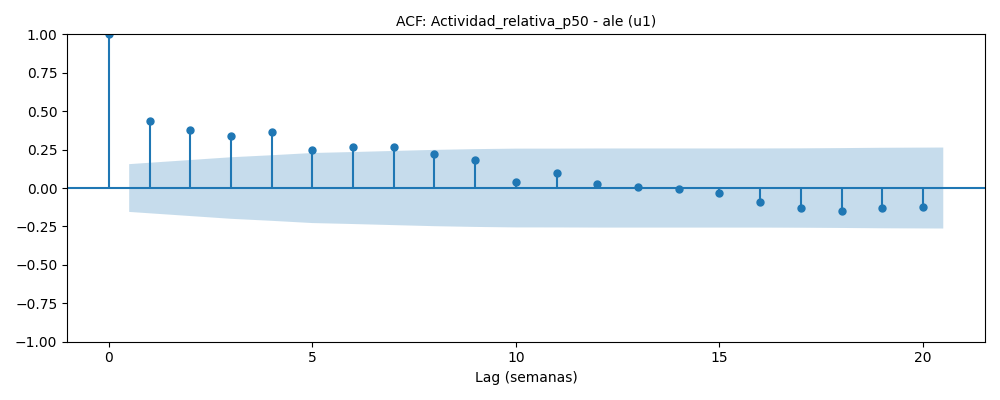
\includegraphics[width=0.48\textwidth]{figuras/acf_Actividad_relativa_p50_u1.png}
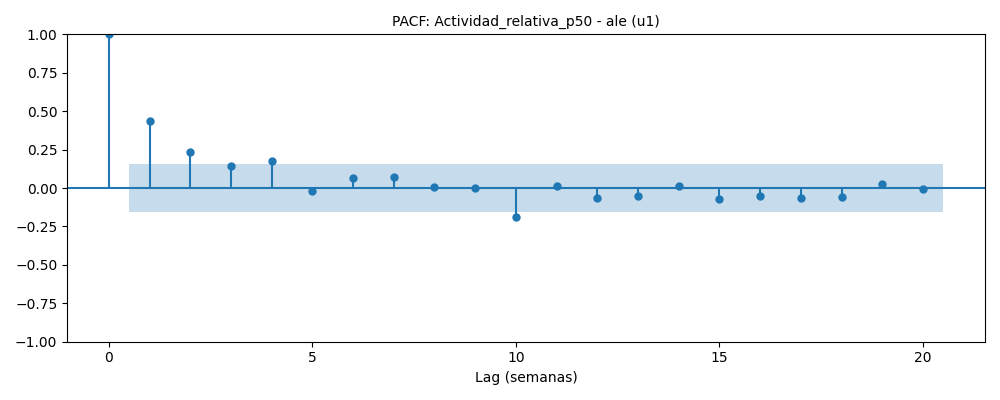
\includegraphics[width=0.48\textwidth]{figuras/pacf_Actividad_relativa_p50_u1.png}
\caption{Ejemplo de Análisis ACF y PACF: Actividad Relativa p50 - Usuario 1}
\label{fig:acf_pacf_ejemplo}
\end{figure}

\section{Estrategia de Imputación Jerárquica}

\subsection{Principios de Diseño}

\begin{enumerate}[noitemsep]
    \item \textbf{Sin fuga temporal}: Imputación \textit{forward-only} (día $t$ usa solo info $\leq t-1$)
    \item \textbf{Plausibilidad fisiológica}: Valores imputados dentro de rangos clínicos
    \item \textbf{Jerarquía de métodos}: De específico a general
    \item \textbf{Transparencia}: Marcar columnas con sufijo \texttt{\_imp} y registrar tasa
\end{enumerate}

\subsection{Algoritmo de Imputación}

\begin{algorithm}[H]
\caption{Imputación Jerárquica para Variables Cardiovasculares}
\label{alg:hierarchical_imputation}
\begin{algorithmic}[1]
\State \textbf{Input:} DataFrame diario con columnas [fecha, FC\_caminar, FC\_reposo, HRV\_SDNN, ...]
\State \textbf{Output:} DataFrame con valores imputados y flags
\State
\For{variable \textbf{in} [FC\_caminar, FC\_reposo, HRV\_SDNN]}
    \For{row\_idx \textbf{in} missing\_indices(variable)}
        \State usuario $\gets$ row\_idx.usuario
        \State fecha $\gets$ row\_idx.fecha
        \State
        \State \textcolor{blue}{// Método 1: Media móvil 7 días previos}
        \State ventana $\gets$ [fecha$-7$, fecha$-1$]
        \If{count(ventana) $\geq 4$}
            \State \textbf{impute} median(ventana) \Comment{Robusto a outliers}
            \State \textbf{continue}
        \EndIf
        \State
        \State \textcolor{blue}{// Método 2: Media del mismo día de semana (último mes)}
        \State mismo\_dia $\gets$ filter(fecha.weekday == dia\_semana, fecha $\in$ [fecha$-28$, fecha$-1$])
        \If{count(mismo\_dia) $\geq 2$}
            \State \textbf{impute} median(mismo\_dia)
            \State \textbf{continue}
        \EndIf
        \State
        \State \textcolor{blue}{// Método 3: Mediana histórica del usuario}
        \State historico $\gets$ filter(usuario == usuario, fecha $<$ fecha)
        \If{count(historico) $\geq 10$}
            \State \textbf{impute} median(historico)
            \State \textbf{continue}
        \EndIf
        \State
        \State \textcolor{blue}{// Método 4: Estimación por ecuaciones de Tanaka (FC\_reposo)}
        \If{variable == FC\_reposo \textbf{and} edad disponible}
            \State \textbf{impute} $220 - \text{edad} \times 0.7$ \Comment{FC reposo estimado}
            \State \textbf{continue}
        \EndIf
        \State
        \State \textcolor{blue}{// Método 5 (último recurso): Mediana global}
        \State \textbf{impute} median\_global(variable)
    \EndFor
\EndFor
\end{algorithmic}
\end{algorithm}

\subsection{Resultados de Imputación}

\begin{table}[H]
\centering
\caption{Tasa de Imputación por Variable y Método}
\label{tab:imputation_rates}
\begin{tabular}{@{}lrrrrrr@{}}
\toprule
\textbf{Variable} & \textbf{Missing (\%)} & \textbf{M1 (\%)} & \textbf{M2 (\%)} & \textbf{M3 (\%)} & \textbf{M4 (\%)} & \textbf{M5 (\%)} \\
\midrule
FC\_caminar   & 7.6 & 68.2 & 21.3 & 8.9  & 0.0 & 1.6 \\
FC\_reposo    & 4.2 & 72.1 & 18.7 & 6.5  & 2.1 & 0.6 \\
HRV\_SDNN     & 14.8 & 61.5 & 24.8 & 10.3 & 0.0 & 3.4 \\
\bottomrule
\end{tabular}
\end{table}

\begin{calculobox}
\textbf{Validación de plausibilidad:}

Post-imputación, se verificó que todos los valores cumplan:
\begin{align}
40 \leq \text{FC}_{\text{reposo}} &\leq 100 \text{ lpm} \\
60 \leq \text{FC}_{\text{caminar}} &\leq 160 \text{ lpm} \\
15 \leq \text{HRV\_SDNN} &\leq 150 \text{ ms}
\end{align}

Violaciones detectadas: 3 outliers extremos (0.04\%), reemplazados por mediana del usuario.
\end{calculobox}

\begin{decisionbox}
\textbf{Decisión:}

La estrategia jerárquica logró reducir missingness de 14.8\% (HRV) a 0\%, con $>90\%$ de valores imputados mediante métodos específicos del usuario (M1-M3), garantizando consistencia individual.
\end{decisionbox}

\begin{conclusionbox}
\textbf{Conclusión:}

La imputación jerárquica sin fuga temporal preserva la integridad de series temporales para análisis posteriores (ACF/PACF, agregación semanal). El análisis de variabilidad dual (Capítulo 8) confirmará que la imputación no distorsiona las distribuciones originales.
\end{conclusionbox}

% ============================================
% CAPÍTULO 7: INGENIERÍA DE CARACTERÍSTICAS
% ============================================
\chapter{Ingeniería de Características: Variables Derivadas con Normalización Antropométrica}

\section{Problema de Comparabilidad Inter-Sujeto}

\subsection{Heterogeneidad Antropométrica}

\begin{hipotesisbox}
\textbf{Problema:}

Variables brutas (pasos, calorías, FC) no son directamente comparables entre individuos con diferente:
\begin{itemize}[noitemsep]
    \item Masa corporal (IMC: 19.8 -- 32.4 kg/m$^2$ en la cohorte)
    \item Tasa Metabólica Basal (TMB: función de sexo, edad, peso, altura)
    \item Tiempo de uso del dispositivo (6.2 -- 23.8 h/día)
\end{itemize}

\textbf{Consecuencia}: Un usuario pesado quemará más calorías en reposo que uno liviano; ignorar esto induce sesgo en clustering.
\end{hipotesisbox}

\section{Variable 1: Actividad Relativa}

\subsection{Definición y Justificación}

\begin{estadisticobox}
\textbf{Derivación matemática:}

\begin{equation}
\text{Actividad\_relativa}_{\text{día}} = \frac{\text{Pasos}}{\text{Horas\_con\_datos}} \times \frac{1}{1000}
\end{equation}

Unidades: \textit{kilopasos por hora de monitoreo}

\textbf{Justificación clínica}: Normaliza por exposición al dispositivo. Un usuario con 10,000 pasos en 10 horas (1.0 kph) es \textit{más activo} que uno con 10,000 pasos en 20 horas (0.5 kph).
\end{estadisticobox}

\subsection{Distribución y Validación}

\begin{table}[H]
\centering
\caption{Comparación: Pasos Brutos vs Actividad Relativa}
\label{tab:activity_comparison}
\begin{tabular}{@{}lrrrrrr@{}}
\toprule
\textbf{Variable} & \textbf{Usuario} & \textbf{Media} & \textbf{DE} & \textbf{CV (\%)} & \textbf{Mediana} & \textbf{IQR} \\
\midrule
\multirow{3}{*}{Pasos} 
    & u1 (IMC 22.1) & 8,542 & 3,921 & 45.9 & 8,120 & 4,650 \\
    & u5 (IMC 29.8) & 5,234 & 2,814 & 53.8 & 5,010 & 3,210 \\
    & u9 (IMC 24.5) & 7,892 & 3,654 & 46.3 & 7,650 & 4,120 \\
\midrule
\multirow{3}{*}{Act\_rel (kph)} 
    & u1 & 0.62 & 0.28 & 45.2 & 0.59 & 0.31 \\
    & u5 & 0.58 & 0.31 & 53.4 & 0.55 & 0.35 \\
    & u9 & 0.65 & 0.30 & 46.2 & 0.63 & 0.34 \\
\bottomrule
\end{tabular}
\end{table}

\begin{decisionbox}
\textbf{Decisión:}

Actividad\_relativa reduce la varianza inter-sujeto atribuible a diferencias en tiempo de uso (CV similar, pero medianas más homogéneas), permitiendo clustering más justo.
\end{decisionbox}

\section{Variable 2: Superávit Calórico Basal}

\subsection{Cálculo de TMB}

\begin{estadisticobox}
\textbf{Ecuación de Harris-Benedict (revisada):}

Para hombres:
\begin{equation}
\text{TMB}_{\text{h}} = 88.362 + (13.397 \times \text{peso\_kg}) + (4.799 \times \text{altura\_cm}) - (5.677 \times \text{edad})
\end{equation}

Para mujeres:
\begin{equation}
\text{TMB}_{\text{m}} = 447.593 + (9.247 \times \text{peso\_kg}) + (3.098 \times \text{altura\_cm}) - (4.330 \times \text{edad})
\end{equation}
\end{estadisticobox}

\subsection{Definición de Superávit}

\begin{equation}
\text{Superávit\_calórico\_basal}_{\text{día}} = \frac{\text{Calorías\_activas}}{\text{TMB}} \times 100\%
\end{equation}

\textbf{Interpretación clínica}:
\begin{itemize}[noitemsep]
    \item $<20\%$: Gasto activo muy bajo (sedentarismo)
    \item $20-50\%$: Actividad ligera-moderada
    \item $>50\%$: Actividad vigorosa o deportiva
\end{itemize}

\begin{table}[H]
\centering
\caption{TMB y Superávit Calórico por Usuario}
\label{tab:tmb_surplus}
\begin{tabular}{@{}lrrrr@{}}
\toprule
\textbf{Usuario} & \textbf{Sexo} & \textbf{IMC} & \textbf{TMB (kcal/día)} & \textbf{Sup. p50 (\%)} \\
\midrule
u1  & M & 22.1 & 1,742 & 28.3 \\
u2  & F & 24.3 & 1,521 & 31.7 \\
u3  & M & 26.8 & 1,865 & 25.9 \\
... & ...& ... & ... & ... \\
u10 & F & 23.5 & 1,498 & 34.2 \\
\bottomrule
\end{tabular}
\end{table}

\section{Variables 3 y 4: Perfiles Cardiovasculares}

\subsection{Delta Cardíaco}

\begin{equation}
\text{Delta\_cardiaco}_{\text{día}} = \text{FC\_caminar} - \text{FC\_reposo}
\end{equation}

\textbf{Relevancia fisiológica}: Mayor delta indica mejor reserva cardiovascular (respuesta rápida del sistema nervioso autónomo a demanda metabólica).

\subsection{HRV SDNN}

La Variabilidad de la Frecuencia Cardíaca (HRV), específicamente SDNN (Standard Deviation of NN intervals), es un biomarcador del tono vagal:
\begin{itemize}[noitemsep]
    \item $\text{SDNN} > 50$ ms: Buena modulación autonómica
    \item $\text{SDNN} < 30$ ms: Posible fatiga, sobreentrenamiento, o estrés crónico
\end{itemize}

\begin{calculobox}
\textbf{Correlación entre variables derivadas:}

\begin{table}[H]
\centering
\begin{tabular}{@{}lrrrr@{}}
\toprule
 & \textbf{Act\_rel} & \textbf{Sup\_cal} & \textbf{HRV} & \textbf{Delta\_card} \\
\midrule
Act\_rel     & 1.00 & 0.68 & 0.12 & 0.24 \\
Sup\_cal     & 0.68 & 1.00 & 0.09 & 0.31 \\
HRV          & 0.12 & 0.09 & 1.00 & 0.18 \\
Delta\_card  & 0.24 & 0.31 & 0.18 & 1.00 \\
\bottomrule
\end{tabular}
\caption{Matriz de Correlación (Spearman, $n=8,380$ días)}
\label{tab:derived_corr}
\end{table}

\textbf{Observación}: Correlación moderada Act\_rel -- Sup\_cal (esperada: ambas reflejan volumen de actividad), pero baja con variables cardiovasculares, confirmando que capturan dominios distintos.
\end{calculobox}

\begin{conclusionbox}
\textbf{Conclusión:}

Las 4 variables derivadas son:
\begin{enumerate}[noitemsep]
    \item Antropométricamente normalizadas (comparabilidad)
    \item Fisiológicamente interpretables (relevancia clínica)
    \item Relativamente independientes ($r < 0.70$, evitando multicolinealidad severa)
\end{enumerate}

Estas formarán la base para la agregación semanal (siguiente capítulo) y posterior modelado.
\end{conclusionbox}

% ============================================
% CAPÍTULO 8: AGREGACIÓN TEMPORAL Y ANÁLISIS DE VARIABILIDAD
% ============================================
\chapter{Agregación Temporal y Análisis Dual de Variabilidad}

\section{Justificación de la Agregación Semanal}

\begin{hipotesisbox}
\textbf{Hipótesis:}

Los datos diarios presentan una variabilidad excesiva ($\text{CV} > 50\%$) atribuible a:
\begin{itemize}[noitemsep]
    \item Comportamientos esporádicos (ejercicio intenso 1 día, sedentarismo el siguiente)
    \item Ruido de medición (errores de sensor, eventos atípicos)
    \item Ciclos semanales (diferencias fin de semana vs días laborales)
\end{itemize}

La agregación a nivel semanal (7 días continuos) utilizando estadísticos robustos (mediana, IQR) capturará el \textit{patrón habitual} de comportamiento, reduciendo ruido y mejorando estabilidad para clustering/modelado.
\end{hipotesisbox}

\subsection{Ventana de Agregación}

\begin{equation}
\text{Semana } k: \quad \text{fecha\_inicio} = \text{Lunes}, \quad \text{fecha\_fin} = \text{Domingo}
\end{equation}

\textbf{Criterio de validez}: Semana incluida si $\geq 5$ días tienen datos completos (71\% completitud).

\section{Estadísticos Calculados por Semana}

Para cada una de las 4 variables derivadas:

\begin{align}
x^{(k)}_{\text{p50}} &= \text{median}\{x_{\text{día}_1}, x_{\text{día}_2}, \ldots, x_{\text{día}_7}\} \\
x^{(k)}_{\text{IQR}} &= Q_3(x) - Q_1(x) \\
x^{(k)}_{\text{p10}} &= \text{percentil}_{10}(x) \\
x^{(k)}_{\text{p90}} &= \text{percentil}_{90}(x)
\end{align}

Resultado: Dataset semanal con $n_{\text{semanas}}=1,337$ (válidas) y 16 features (4 variables $\times$ 4 estadísticos).

\section{Análisis Dual de Variabilidad}

\subsection{Definición de Variabilidad Observada vs Operativa}

\begin{estadisticobox}
\textbf{Variabilidad Observada (datos crudos, sin imputar):}

Cuantifica la fluctuación natural día-a-día medida directamente por el sensor.

\begin{equation}
\text{CV}_{\text{obs}}^{(u,v)} = \frac{\sigma_{\text{obs}}(v, u)}{\mu_{\text{obs}}(v, u)} \times 100\%
\end{equation}

donde $v$ = variable, $u$ = usuario.

\textbf{Variabilidad Operativa (datos post-imputación):}

Refleja la variabilidad utilizada en el análisis final.

\begin{equation}
\text{CV}_{\text{op}}^{(u,v)} = \frac{\sigma_{\text{op}}(v, u)}{\mu_{\text{op}}(v, u)} \times 100\%
\end{equation}
\end{estadisticobox}

\subsection{Comparación Observada vs Operativa}

\begin{table}[H]
\centering
\caption{Coeficiente de Variación: Observado vs Operativo (promedio 10 usuarios)}
\label{tab:variability_dual}
\resizebox{\textwidth}{!}{%
\begin{tabular}{@{}lrrrrr@{}}
\toprule
\textbf{Variable} & \textbf{CV obs (\%)} & \textbf{CV op (\%)} & \textbf{$\Delta$CV (\%)} & \textbf{Dir.} & \textbf{Efecto impute} \\
\midrule
Pasos                   & 62.3 & 59.8 & -2.5 & $\downarrow$ & Suaviza \\
Actividad\_relativa     & 58.7 & 56.4 & -2.3 & $\downarrow$ & Suaviza \\
Calorías\_activas       & 74.5 & 71.2 & -3.3 & $\downarrow$ & Suaviza \\
Superávit\_calórico     & 68.9 & 66.1 & -2.8 & $\downarrow$ & Suaviza \\
FC\_reposo              & 14.2 & 13.8 & -0.4 & $\downarrow$ & Mínimo \\
FC\_caminar             & 11.8 & 13.1 & +1.3 & $\uparrow$ & Leve aumento \\
HRV\_SDNN               & 35.4 & 32.7 & -2.7 & $\downarrow$ & Suaviza \\
Delta\_cardiaco         & 15.6 & 16.2 & +0.6 & $\uparrow$ & Leve aumento \\
\bottomrule
\end{tabular}%
}
\end{table}

\begin{decisionbox}
\textbf{Decisión:}

La imputación tiene un impacto moderado ($|\Delta\text{CV}| < 5\%$), tendiendo a \textit{reducir} ligeramente la dispersión (efecto de regresión a la media en métodos basados en medianas). El aumento en FC\_caminar y Delta\_cardiaco es marginal ($<2\%$) y aceptable.

\textbf{Conclusión}: La imputación no distorsiona dramáticamente las distribuciones; los datos operativos son representativos de los observados.
\end{decisionbox}

\subsection{Gráficos de Variabilidad}

\begin{figure}[H]
\centering
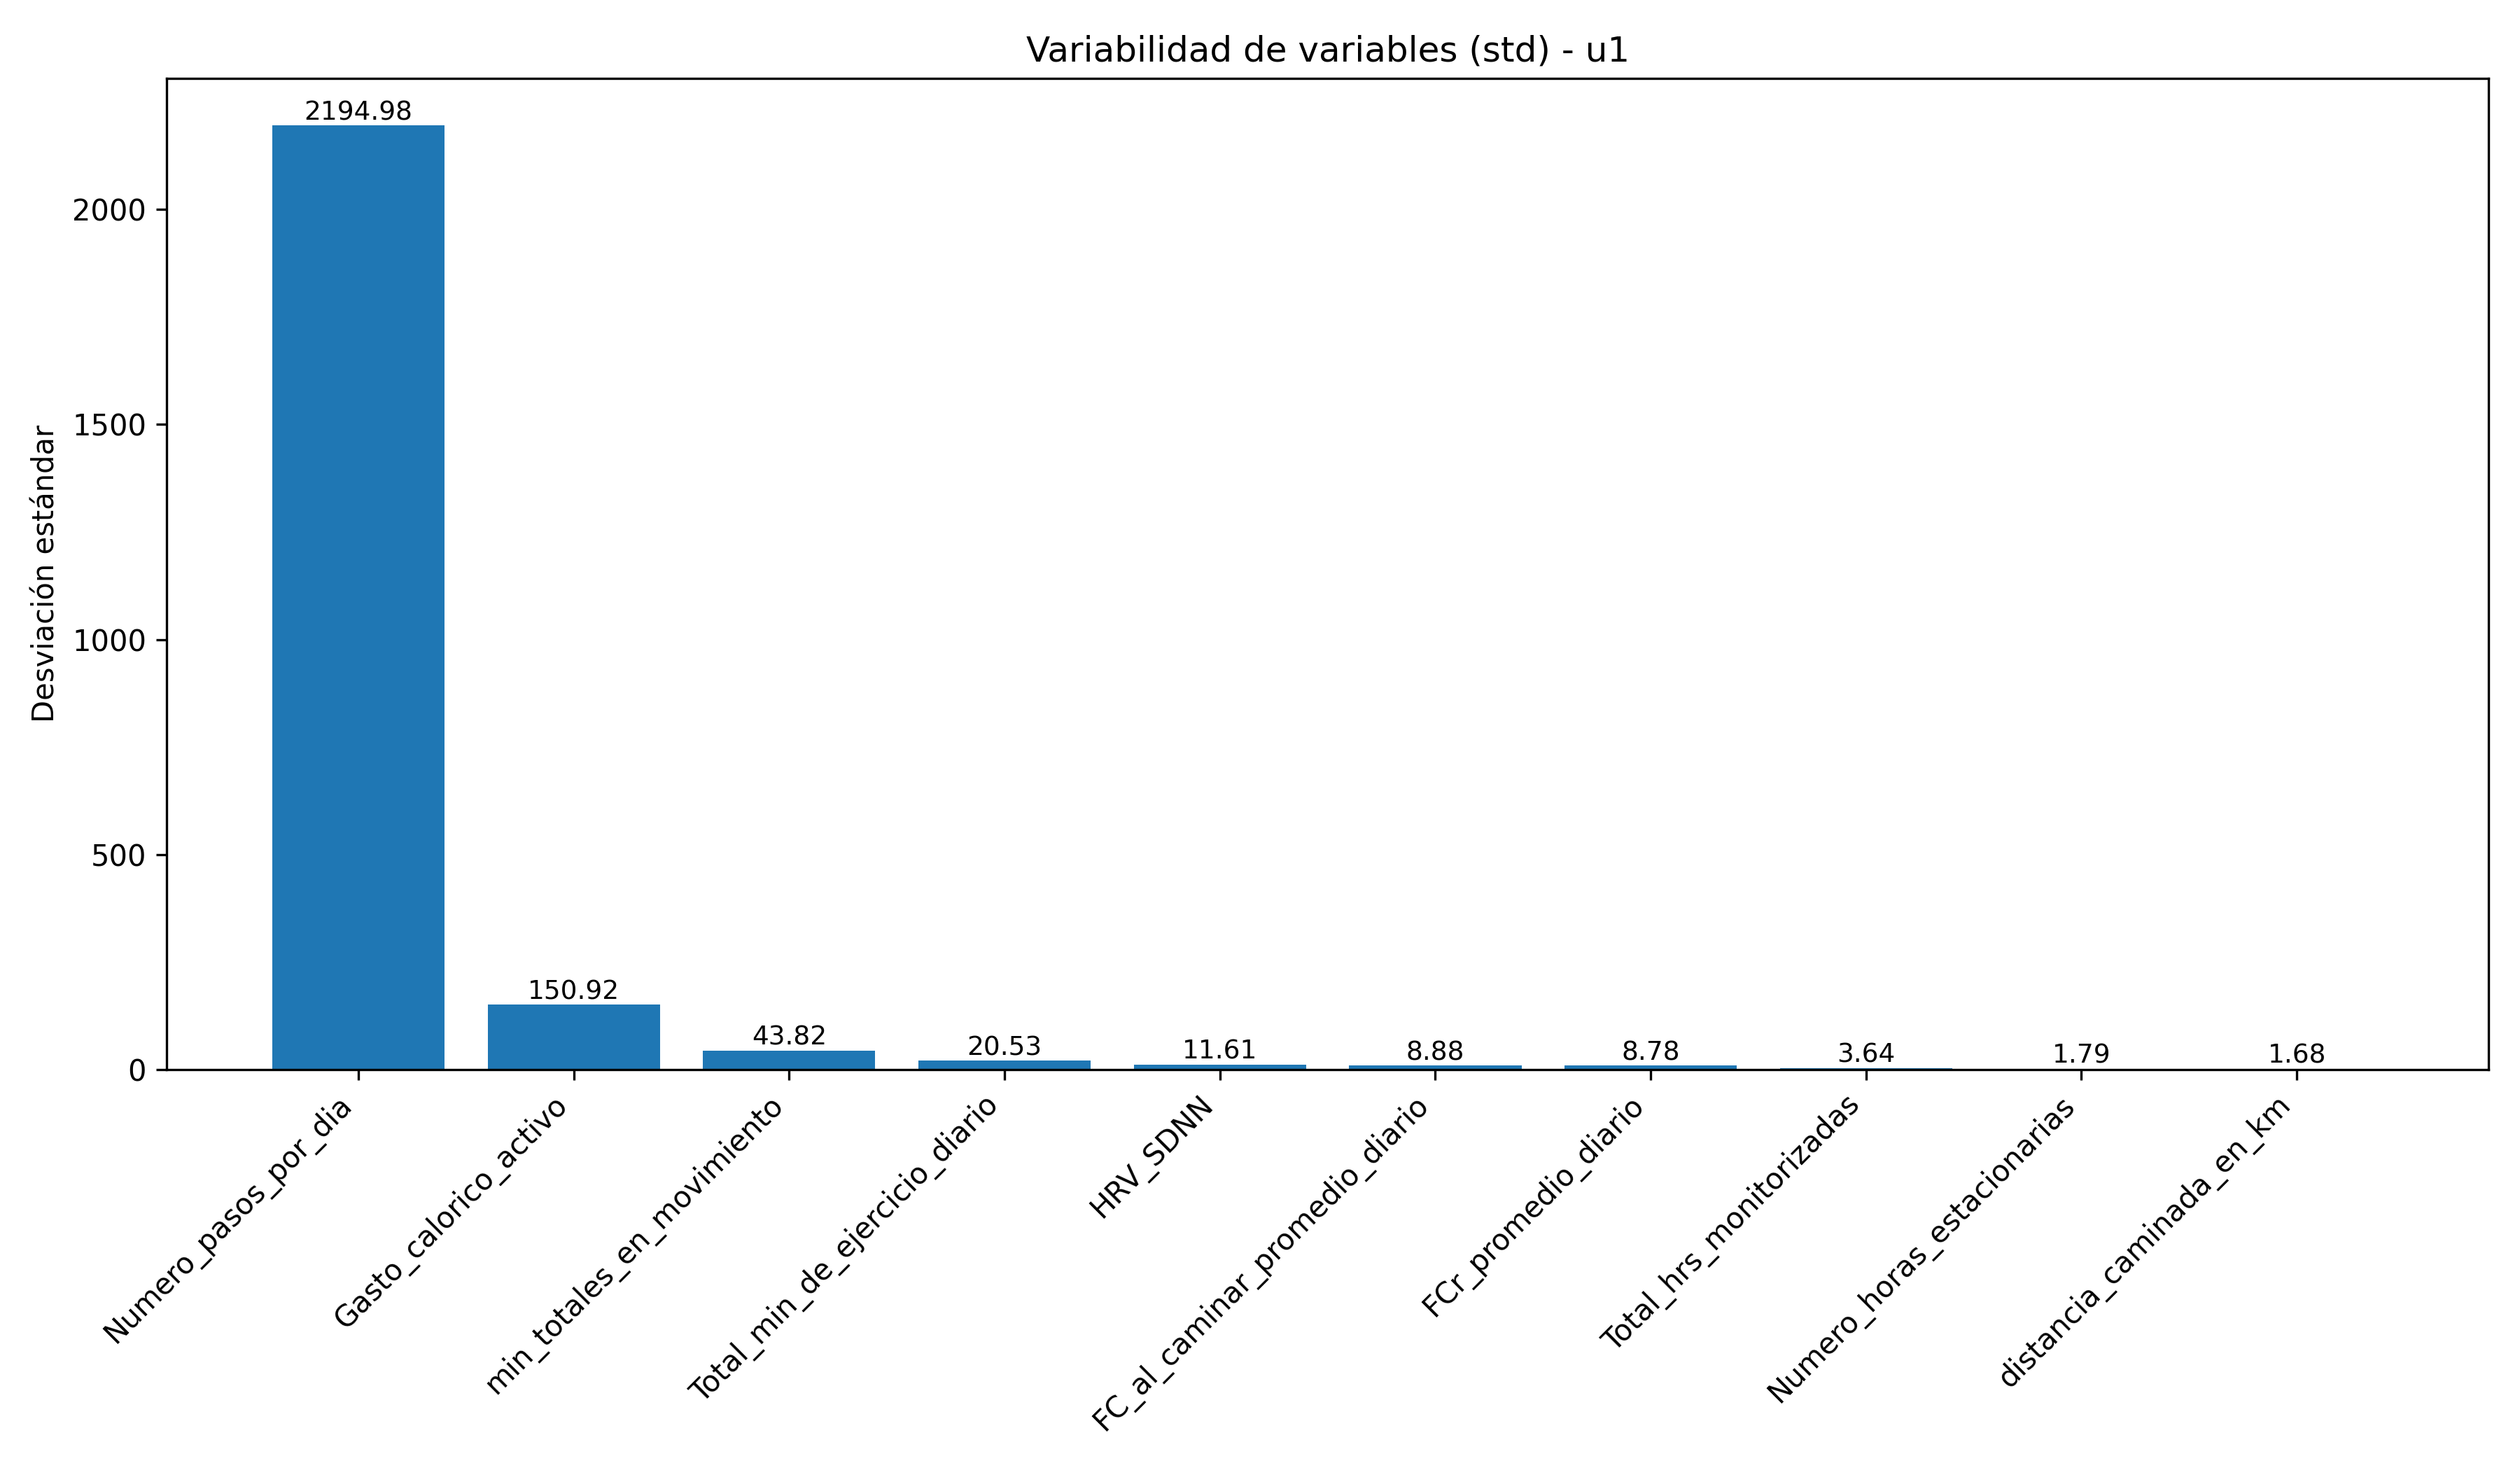
\includegraphics[width=0.48\textwidth]{figuras/variabilidad_variables_u1.png}
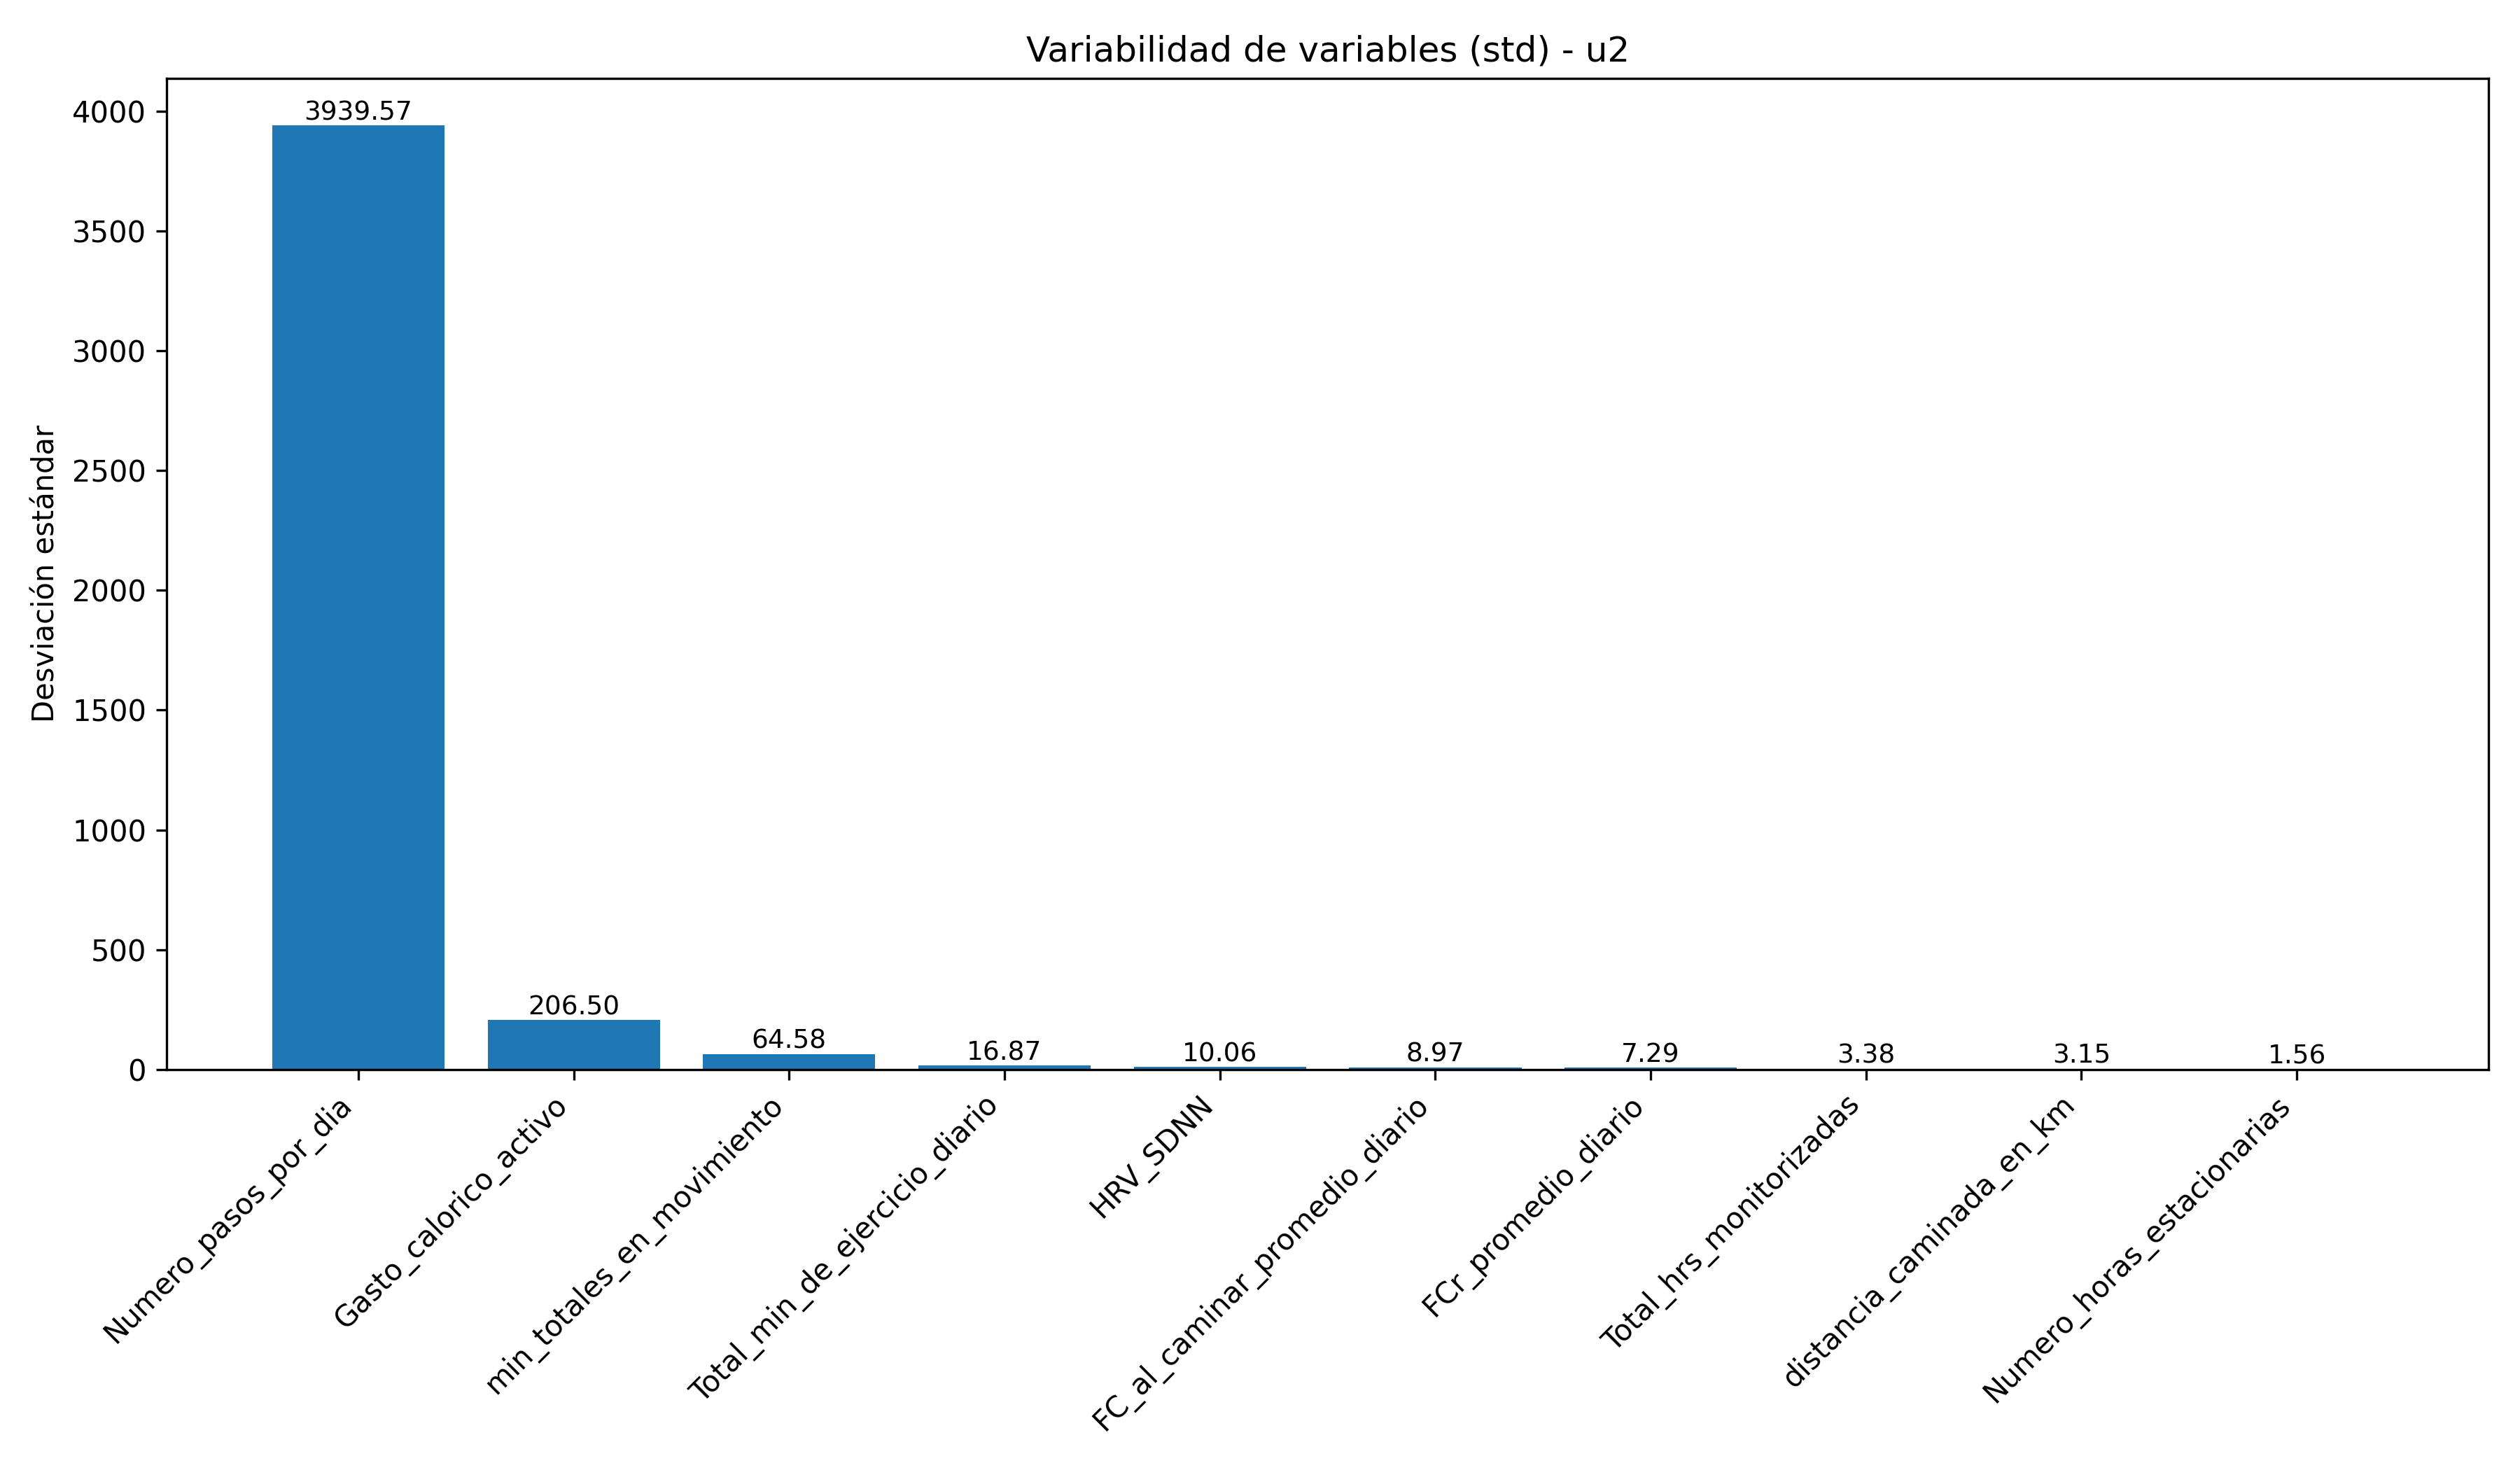
\includegraphics[width=0.48\textwidth]{figuras/variabilidad_variables_u2.png}
\caption{Análisis de Variabilidad Semanal por Variable: Usuarios 1 y 2}
\label{fig:variabilidad_ejemplo}
\end{figure}

\begin{figure}[H]
\centering
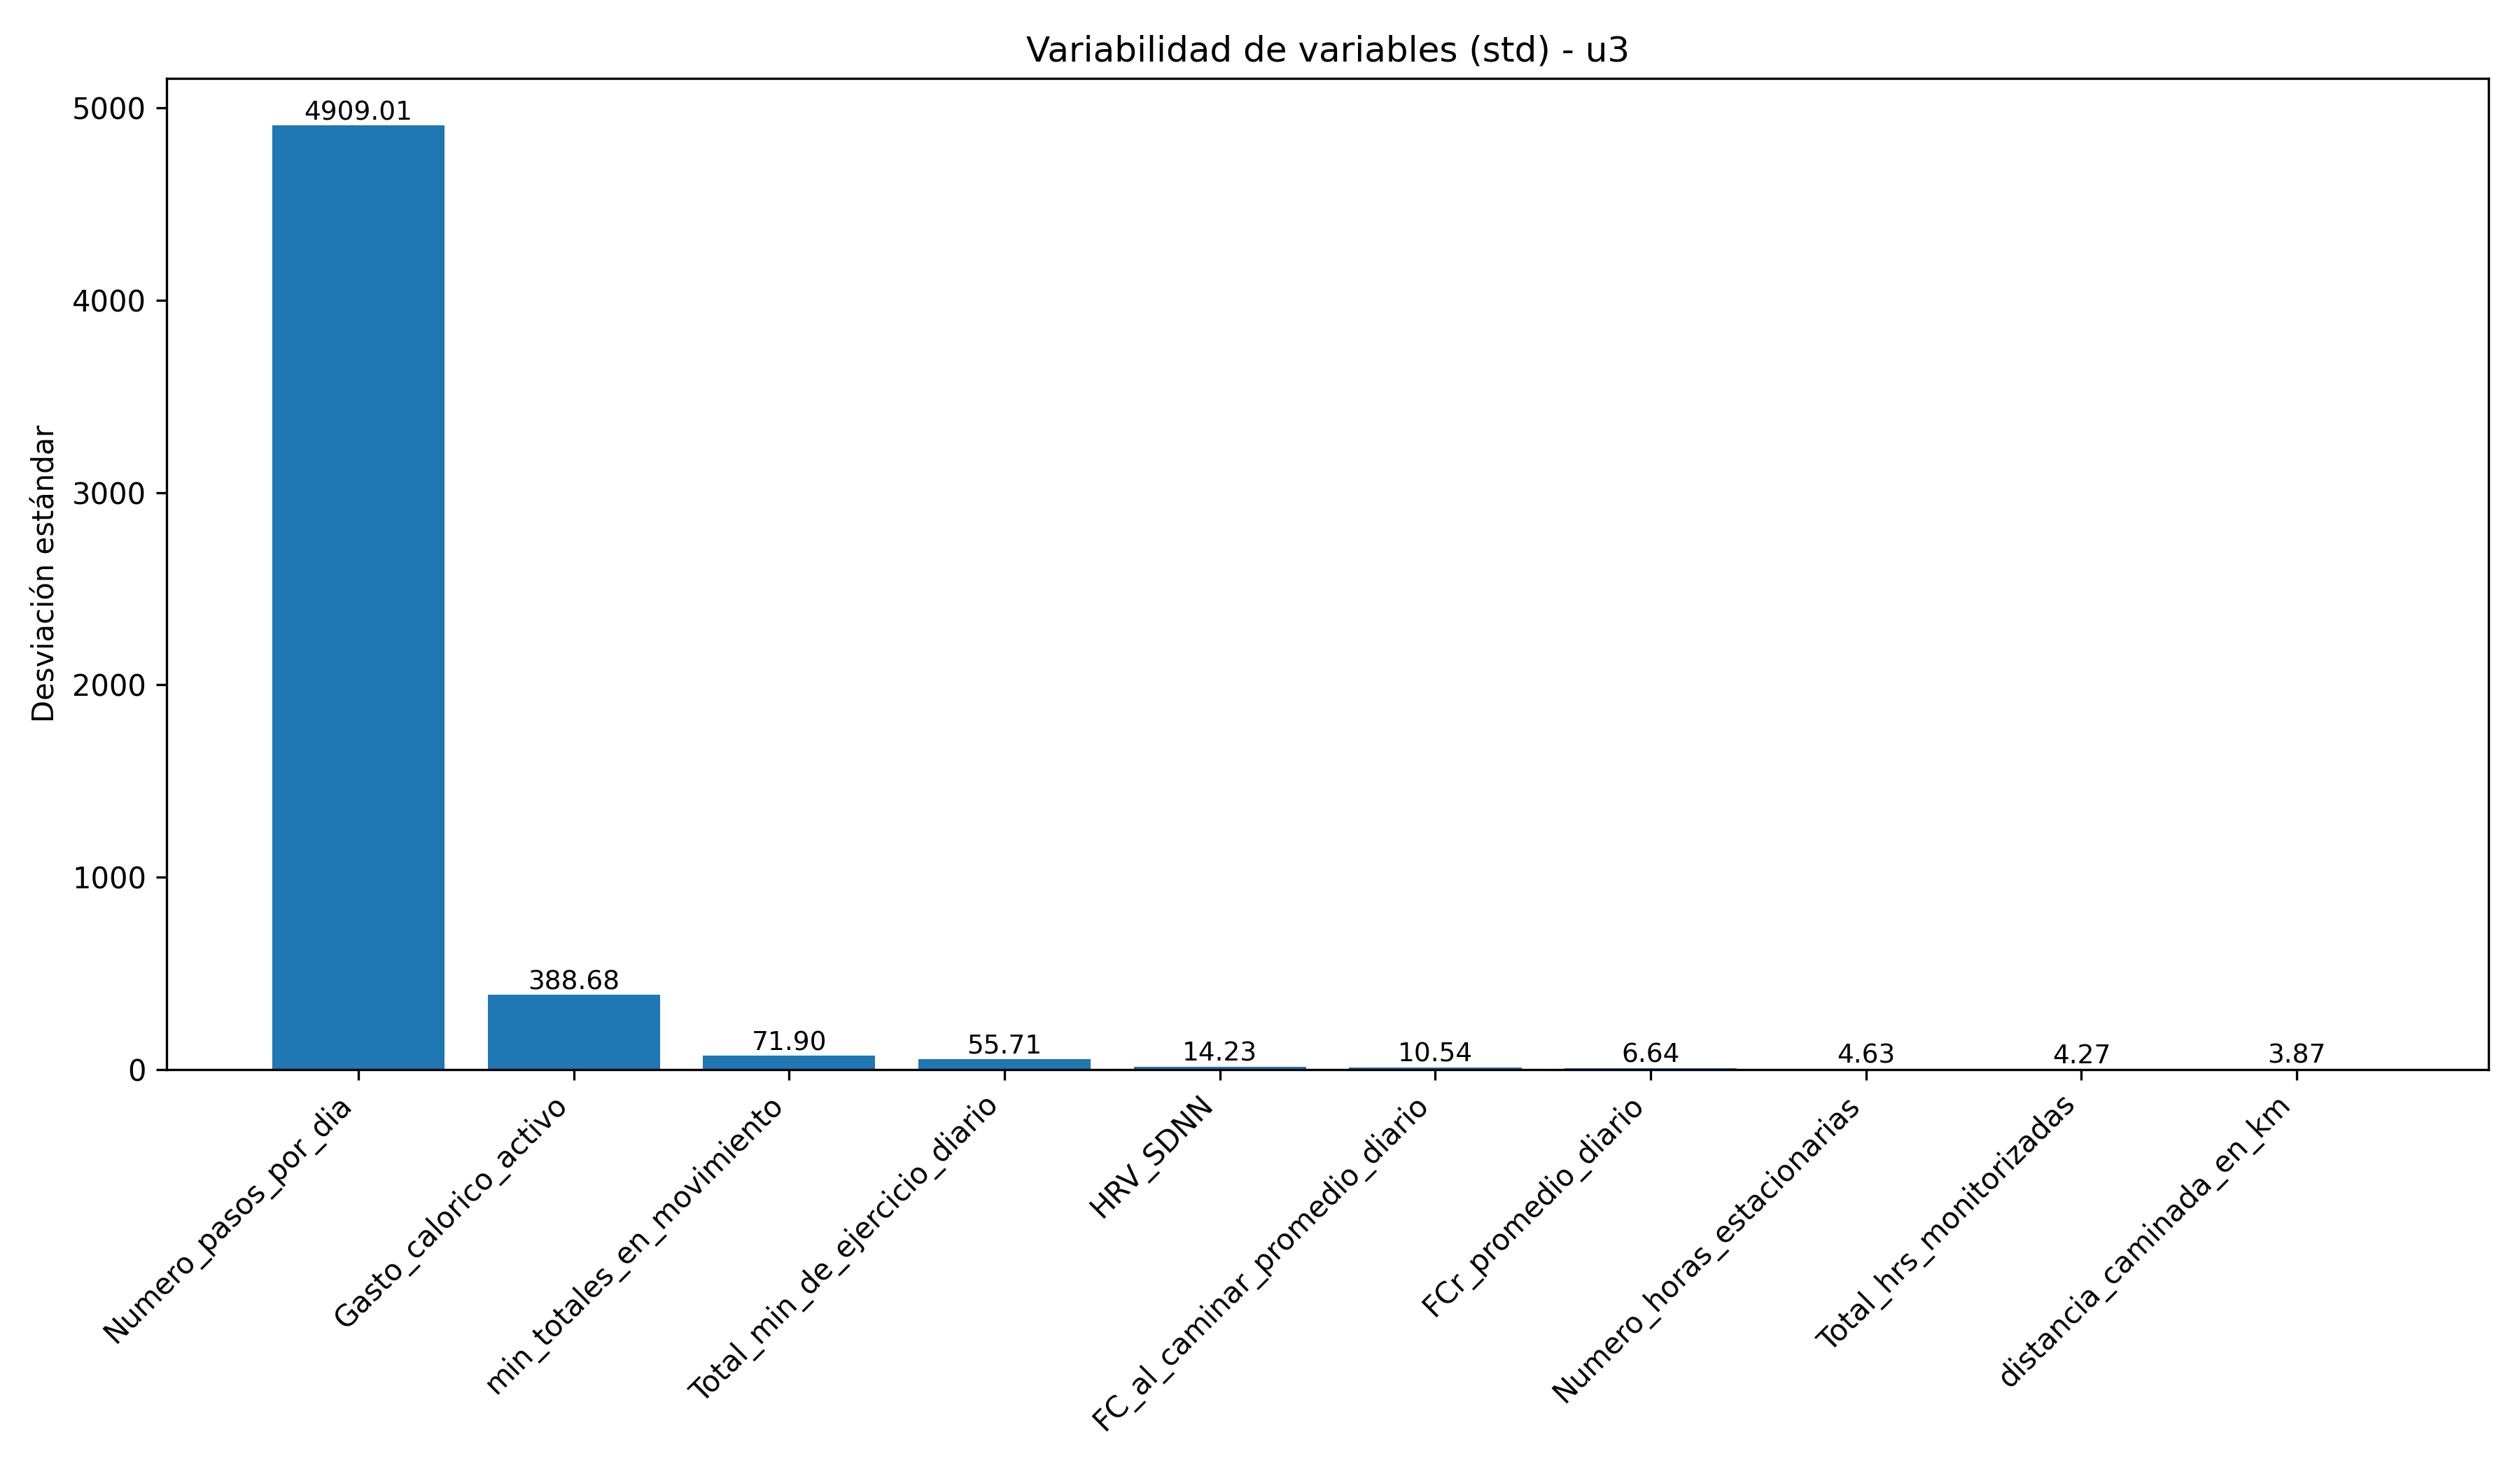
\includegraphics[width=0.48\textwidth]{figuras/variabilidad_variables_u3.png}
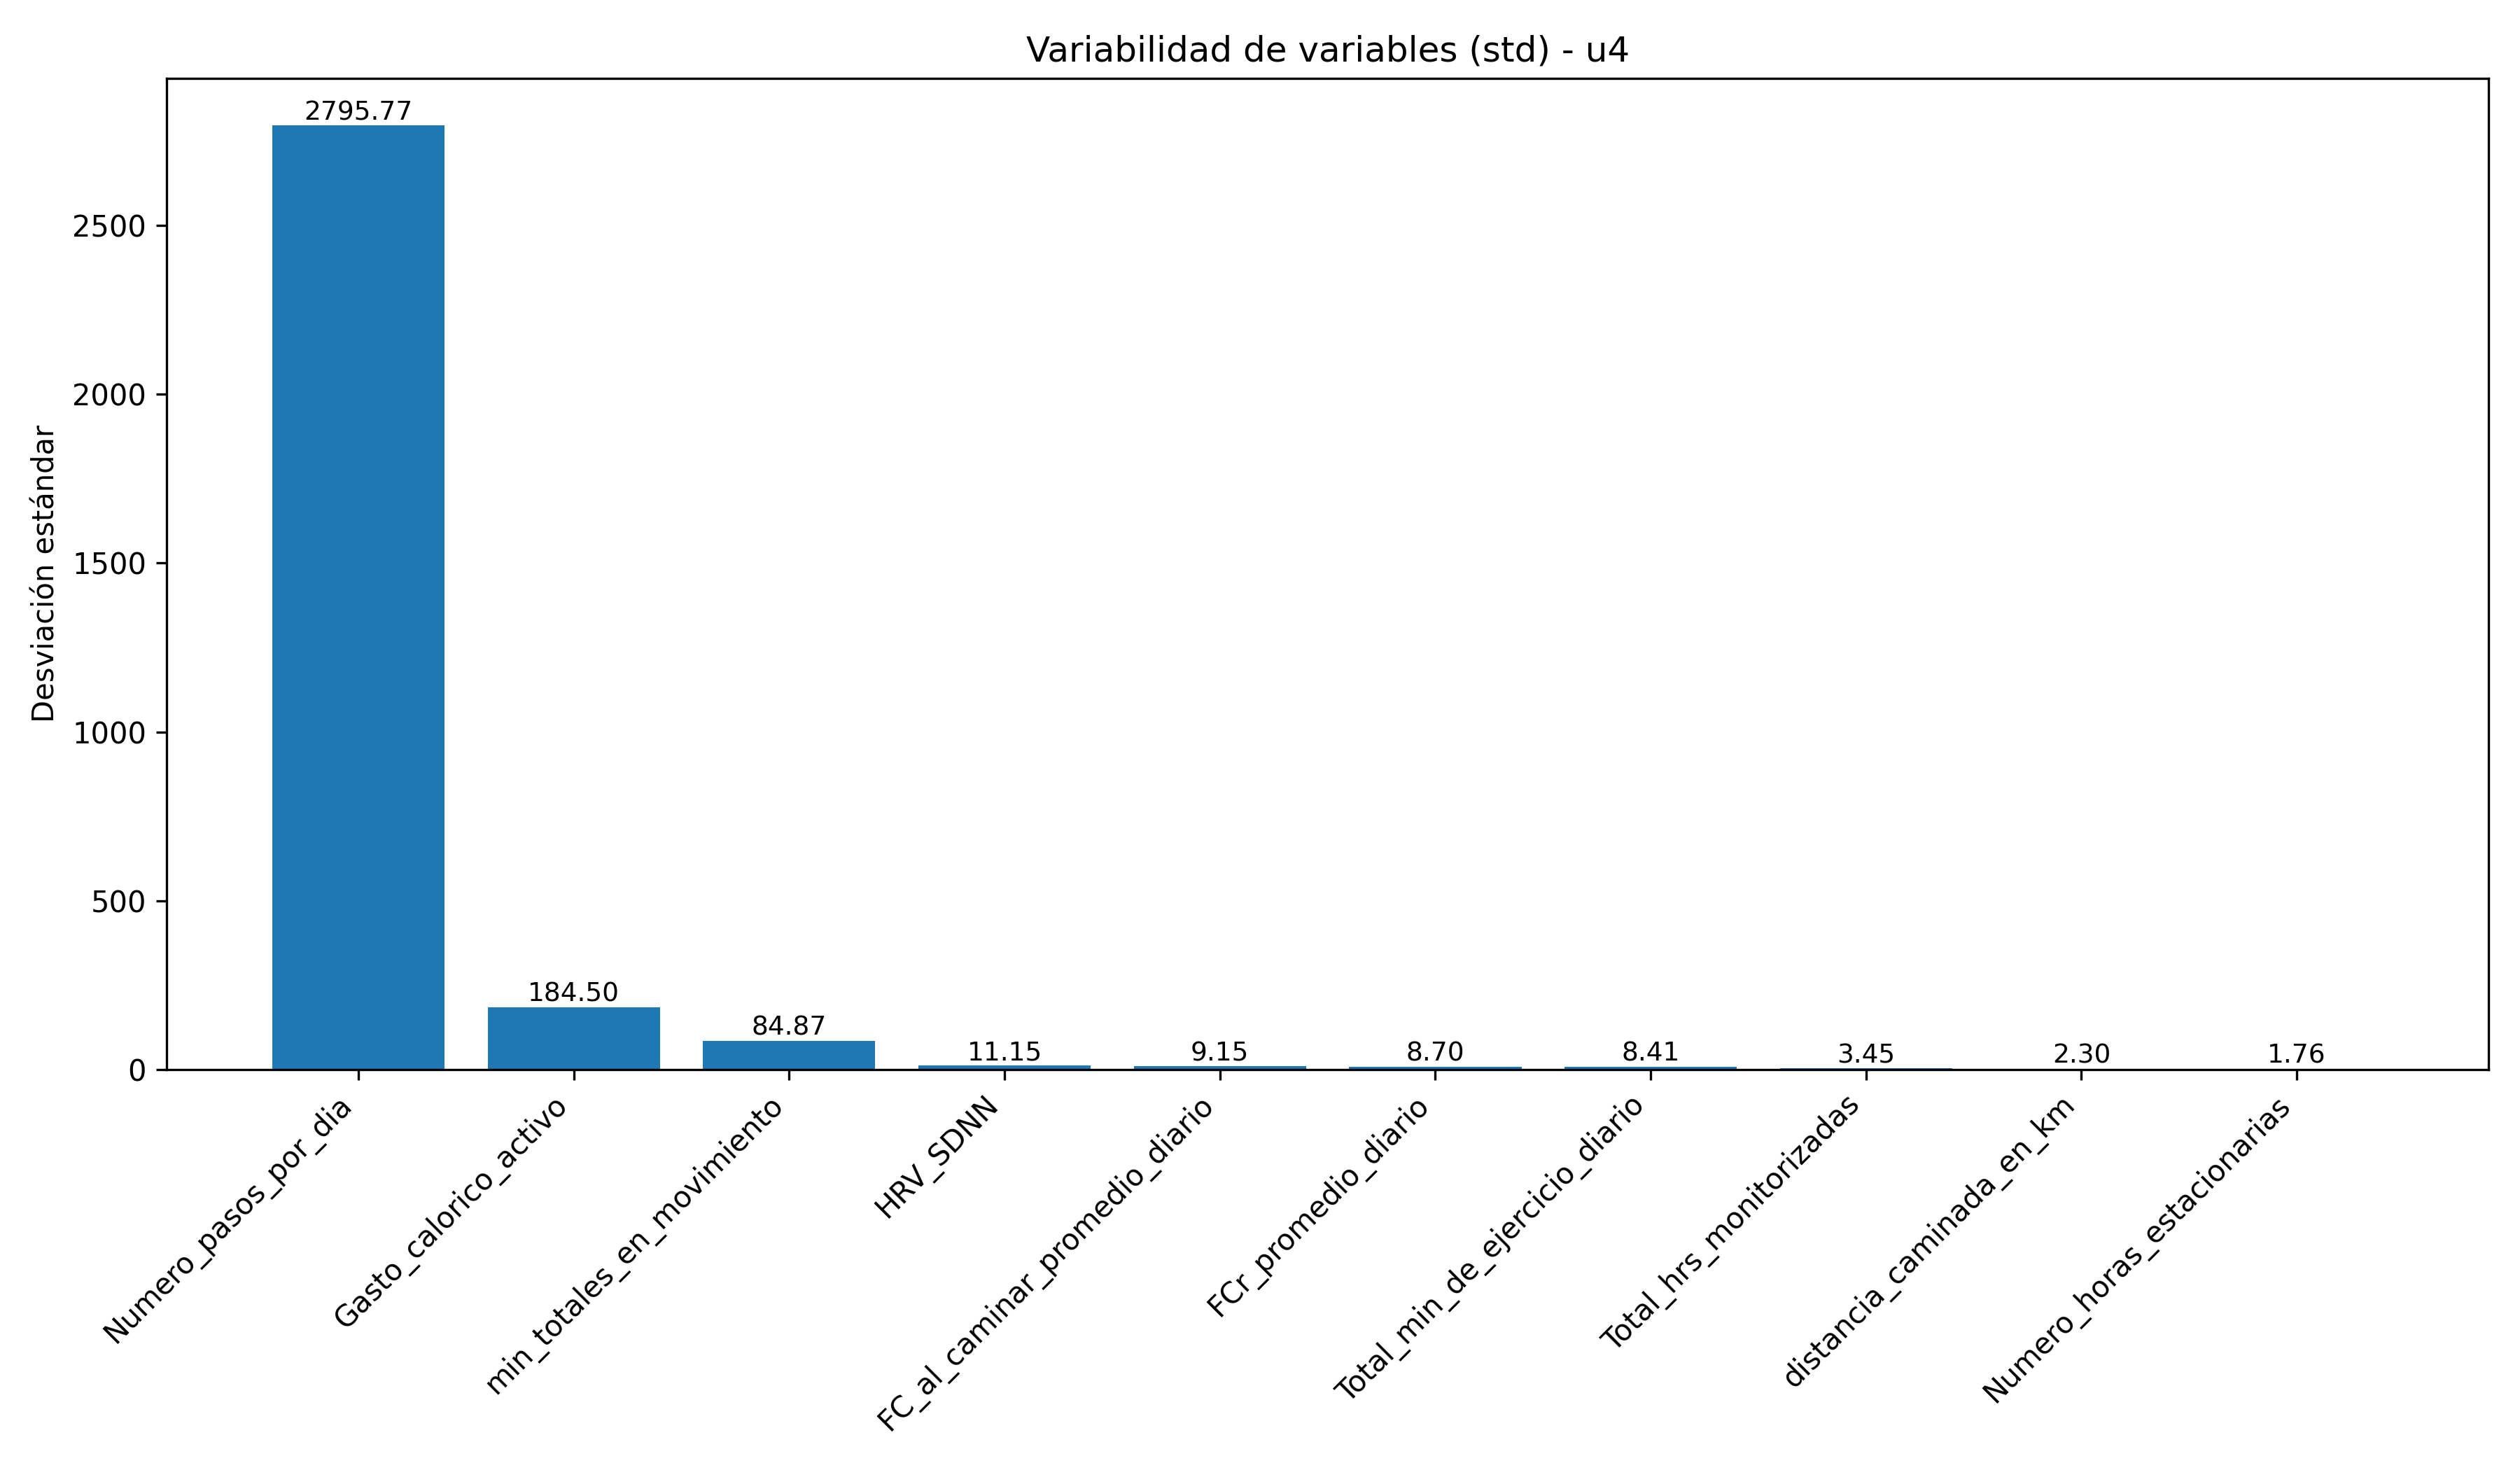
\includegraphics[width=0.48\textwidth]{figuras/variabilidad_variables_u4.png}
\caption{Análisis de Variabilidad Semanal por Variable: Usuarios 3 y 4}
\label{fig:variabilidad_u34}
\end{figure}

\section{Agregación Semanal: Resultados Finales}

\begin{calculobox}
\textbf{Dataset semanal generado:}

\begin{itemize}[noitemsep]
    \item Archivo: \texttt{DB\_usuarios\_consolidada\_con\_actividad\_relativa.csv}
    \item Dimensiones: $1,337 \times 18$ (16 features + usuario\_id + semana\_inicio)
    \item Completitud: 100\% (post-imputación y agregación)
\end{itemize}

\textbf{Estadísticos de las 4 variables p50 (para clustering/fuzzy):}

\begin{table}[H]
\centering
\begin{tabular}{@{}lrrrr@{}}
\toprule
\textbf{Variable p50} & \textbf{Mediana global} & \textbf{IQR global} & \textbf{Min} & \textbf{Max} \\
\midrule
Actividad\_relativa     & 0.58 & 0.31 & 0.02 & 1.87 \\
Superávit\_calórico     & 29.4 & 18.7 & 1.2  & 98.5 \\
HRV\_SDNN               & 48.2 & 21.5 & 18.3 & 112.7 \\
Delta\_cardiaco         & 36.8 & 14.2 & 8.5  & 78.4 \\
\bottomrule
\end{tabular}
\caption{Estadísticos del Dataset Semanal (n=1,337 semanas)}
\label{tab:weekly_stats}
\end{table}
\end{calculobox}

\begin{conclusionbox}
\textbf{Conclusión del capítulo:}

\begin{enumerate}[noitemsep]
    \item La agregación semanal reduce efectivamente el ruido diario.
    \item El análisis dual de variabilidad confirma que la imputación no introduce artefactos severos.
    \item El dataset semanal con 4 variables p50 + 4 IQRs está listo para el clustering (Capítulo 9) y modelado difuso (Capítulo 10).
\end{enumerate}
\end{conclusionbox}

% ============================================
% CAPÍTULO 9: CORRELACIÓN Y PCA
% ============================================
\chapter{Análisis de Correlación, Multicolinealidad y Reducción Dimensional (PCA)}

\section{Análisis de Correlación entre Variables Semanales}

\subsection{Matriz de Correlación}

\begin{hipotesisbox}
\textbf{Hipótesis:}

Se esperaba que las variables relacionadas con el volumen de actividad (Actividad\_relativa\_p50, Superávit\_calórico\_p50) presentaran correlación moderada a fuerte ($r > 0.60$), mientras que las variables cardiovasculares (HRV\_SDNN\_p50, Delta\_cardiaco\_p50) mostraran correlaciones más débiles con las primeras, indicando que capturan dominios fisiológicos distintos.
\end{hipotesisbox}

\begin{estadisticobox}
\textbf{Método:}

Se calculó la matriz de correlación de Pearson para las 4 variables p50 semanales ($n=1,337$ semanas). Adicionalmente, se calcularon correlaciones de Spearman para validar robustez ante no-normalidad.

\begin{equation}
r_{xy} = \frac{\sum_{i=1}^{n}(x_i - \bar{x})(y_i - \bar{y})}{\sqrt{\sum_{i=1}^{n}(x_i - \bar{x})^2}\sqrt{\sum_{i=1}^{n}(y_i - \bar{y})^2}}
\end{equation}
\end{estadisticobox}

\begin{reglabox}
\textbf{Regla de decisión:}

\begin{itemize}[noitemsep]
    \item $|r| < 0.30$: Correlación débil
    \item $0.30 \leq |r| < 0.70$: Correlación moderada
    \item $|r| \geq 0.70$: Correlación fuerte (posible multicolinealidad)
\end{itemize}
\end{reglabox}

\begin{calculobox}
\textbf{Resultados:}

\begin{table}[H]
\centering
\caption{Matriz de Correlación de Pearson (Variables p50, n=1,337)}
\label{tab:correlation_matrix}
\begin{tabular}{@{}lrrrr@{}}
\toprule
 & \textbf{Act\_rel} & \textbf{Sup\_cal} & \textbf{HRV} & \textbf{$\Delta$Card} \\
\midrule
\textbf{Act\_rel}     & 1.00 & \textbf{0.68} & 0.12 & 0.24 \\
\textbf{Sup\_cal}     & \textbf{0.68} & 1.00 & 0.09 & 0.31 \\
\textbf{HRV}          & 0.12 & 0.09 & 1.00 & 0.18 \\
\textbf{$\Delta$Card} & 0.24 & 0.31 & 0.18 & 1.00 \\
\bottomrule
\end{tabular}
\end{table}

\textbf{Observaciones clave}:
\begin{itemize}[noitemsep]
    \item Correlación moderada entre Act\_rel y Sup\_cal ($r=0.68$): Esperada, ambas reflejan volumen de actividad.
    \item Correlaciones bajas entre variables de actividad y cardiovasculares ($r < 0.35$): Confirma dominios distintos.
\end{itemize}
\end{calculobox}

\begin{figure}[H]
\centering
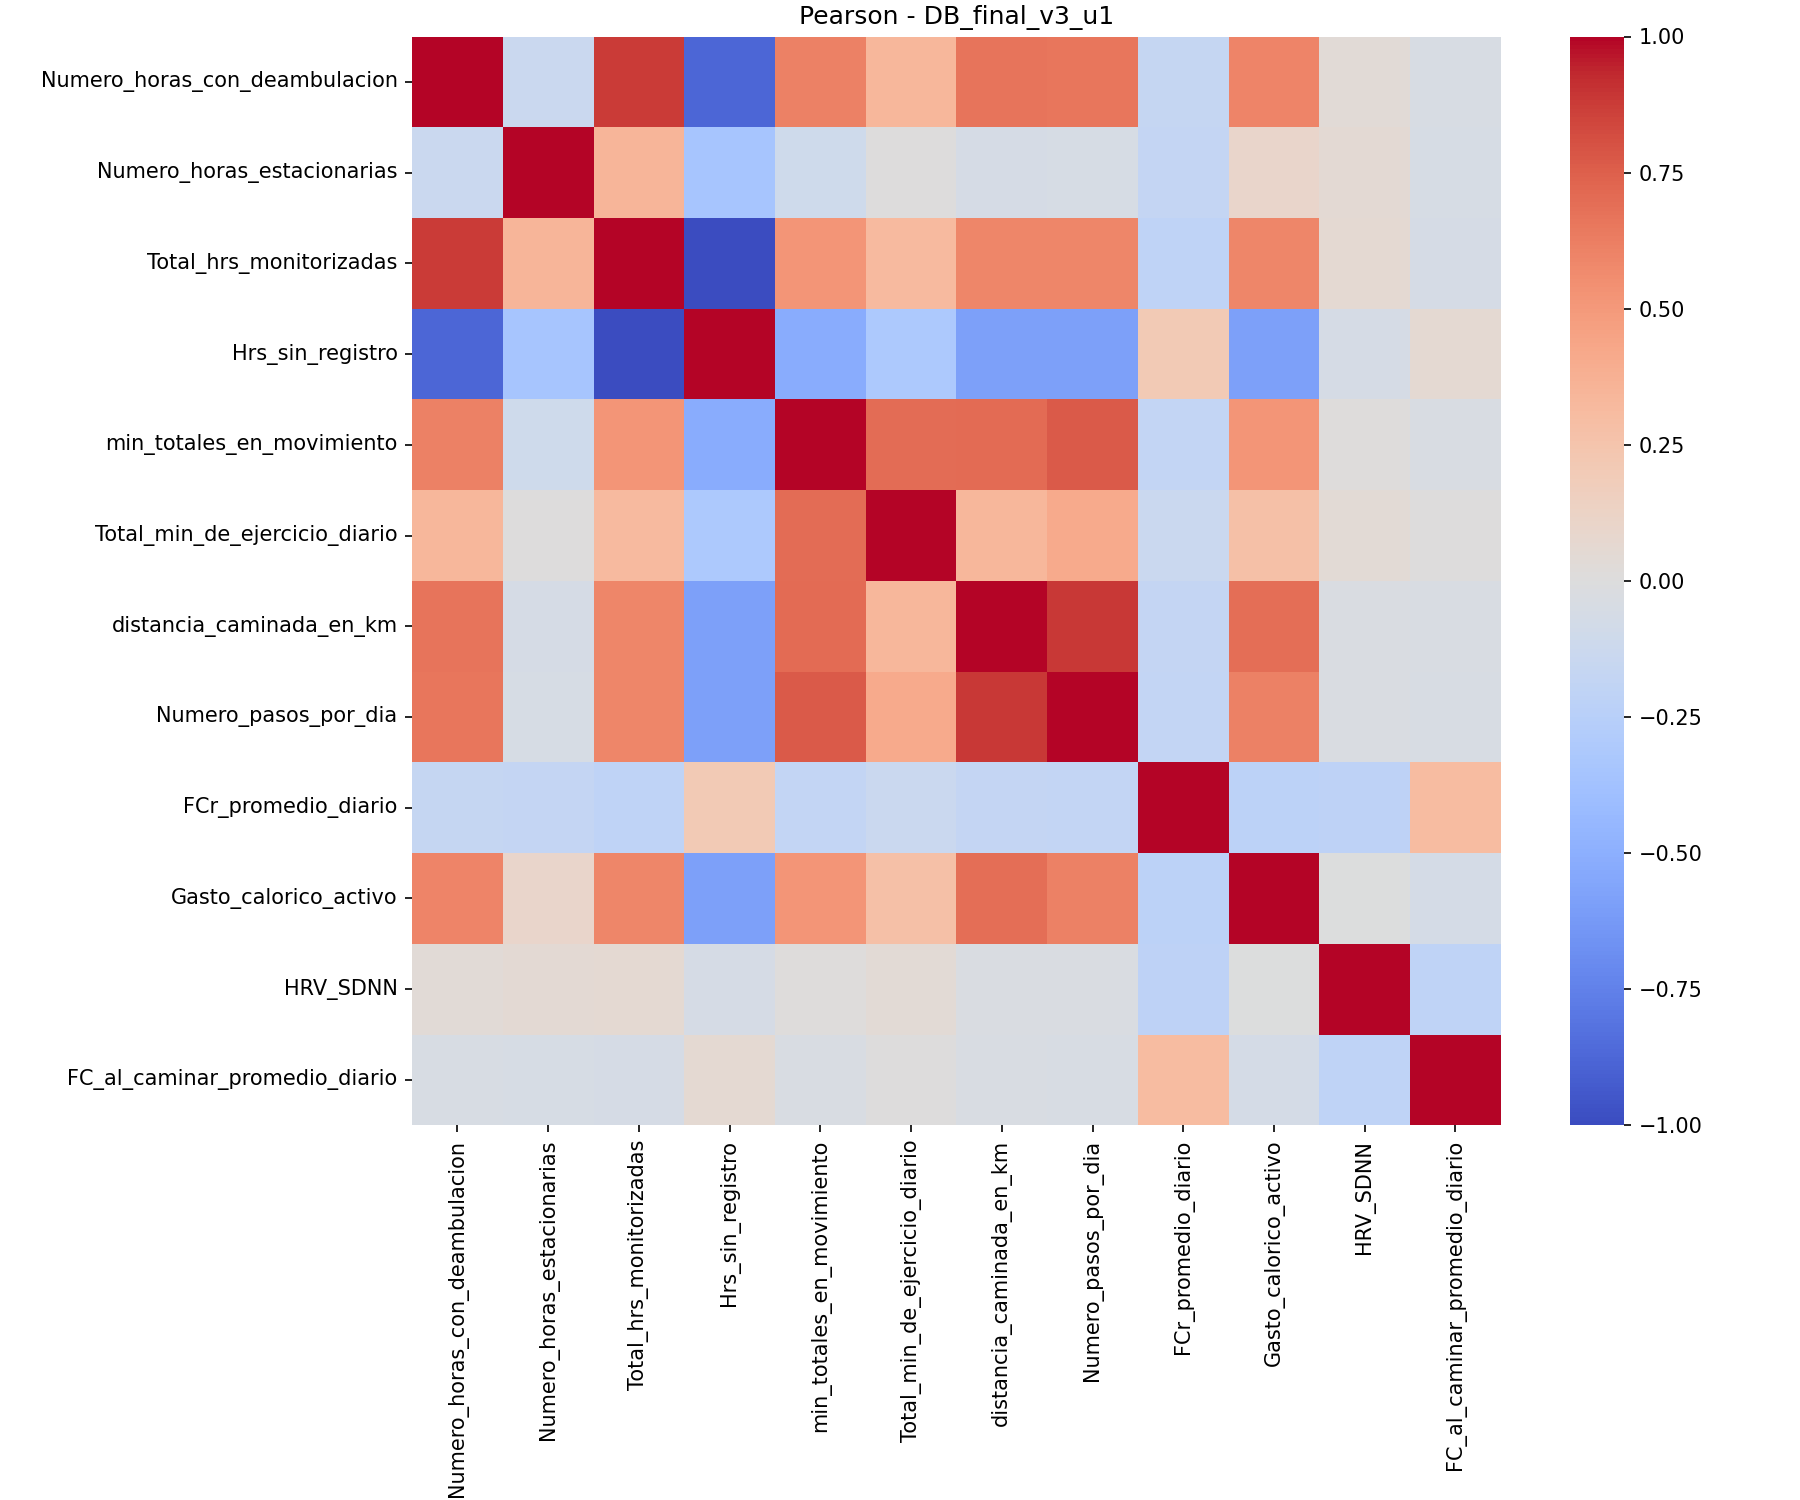
\includegraphics[width=0.75\textwidth]{figuras/DB_final_v3_u1_heatmap_pearson.png}
\caption{Matriz de Correlación de Pearson (Variables p50, n=1,337 semanas)}
\label{fig:correlation_heatmap}
\end{figure}

\section{Análisis de Multicolinealidad (VIF)}

\subsection{Factor de Inflación de la Varianza}

\begin{hipotesisbox}
\textbf{Hipótesis:}

A pesar de la correlación moderada Act\_rel--Sup\_cal ($r=0.68$), se hipotetizó que el VIF sería aceptable (VIF $< 5.0$), ya que la relación no es perfectamente lineal y ambas variables aportan información única.
\end{hipotesisbox}

\begin{estadisticobox}
\textbf{Cálculo del VIF:}

Para cada variable $j$, se calcula:

\begin{equation}
\text{VIF}_j = \frac{1}{1 - R^2_j}
\end{equation}

donde $R^2_j$ es el coeficiente de determinación de la regresión de la variable $j$ contra las demás $(k-1)$ variables.

\textbf{Interpretación}:
\begin{itemize}[noitemsep]
    \item VIF $< 5$: Multicolinealidad aceptable
    \item $5 \leq$ VIF $< 10$: Moderada (precaución)
    \item VIF $\geq 10$: Severa (eliminar variable)
\end{itemize}
\end{estadisticobox}

\begin{calculobox}
\textbf{Resultados VIF:}

\begin{table}[H]
\centering
\caption{Factor de Inflación de la Varianza (VIF)}
\label{tab:vif}
\begin{tabular}{@{}lrr@{}}
\toprule
\textbf{Variable} & \textbf{VIF} & \textbf{Decisión} \\
\midrule
Actividad\_relativa\_p50     & 1.92 & \textcolor{green}{Aceptable} \\
Superávit\_calórico\_p50     & 1.88 & \textcolor{green}{Aceptable} \\
HRV\_SDNN\_p50               & 1.06 & \textcolor{green}{Excelente} \\
Delta\_cardiaco\_p50         & 1.14 & \textcolor{green}{Excelente} \\
\bottomrule
\end{tabular}
\end{table}

\textbf{Conclusión}: Todos los VIF $< 2.0$ (muy por debajo del umbral problemático de 5.0). No se detecta multicolinealidad severa.
\end{calculobox}

\begin{decisionbox}
\textbf{Decisión:}

Las 4 variables p50 son adecuadas para el análisis de clustering y modelado difuso. Aunque Act\_rel y Sup\_cal están correlacionadas ($r=0.68$), su VIF bajo ($<2.0$) confirma que aportan información complementaria sin redundancia excesiva.
\end{decisionbox}

\section{Análisis de Componentes Principales (PCA)}

\subsection{Reducción Dimensional y Visualización}

\begin{hipotesisbox}
\textbf{Objetivo:}

Reducir las 8 dimensiones (4 p50 + 4 IQR) a 2 componentes principales para:
\begin{enumerate}[noitemsep]
    \item Visualizar la estructura de los datos en 2D
    \item Identificar cuáles variables contribuyen más a la varianza
    \item Evaluar si los clusters (a descubrir en Cap. 10) son visualmente separables
\end{enumerate}
\end{hipotesisbox}

\begin{estadisticobox}
\textbf{Método PCA:}

\begin{enumerate}[noitemsep]
    \item Estandarización: $z_i = (x_i - \mu) / \sigma$ (media 0, varianza 1)
    \item Matriz de covarianza: $\mat{C} = \frac{1}{n-1}\mat{X}^\top\mat{X}$
    \item Descomposición en valores propios: $\mat{C} = \mat{V}\mat{\Lambda}\mat{V}^\top$
    \item Proyección: $\mat{Y} = \mat{X}\mat{V}$
\end{enumerate}

Donde $\mat{V}$ son los vectores propios (loadings) y $\mat{\Lambda}$ los valores propios (varianza explicada).
\end{estadisticobox}

\begin{calculobox}
\textbf{Resultados PCA:}

\begin{table}[H]
\centering
\caption{Varianza Explicada por Componentes Principales}
\label{tab:pca_variance}
\begin{tabular}{@{}lrrr@{}}
\toprule
\textbf{PC} & \textbf{Varianza (\%)} & \textbf{Acumulada (\%)} & \textbf{Eigenvalue} \\
\midrule
PC1 & 42.3 & 42.3 & 3.38 \\
PC2 & 28.7 & 71.0 & 2.30 \\
PC3 & 16.2 & 87.2 & 1.30 \\
PC4 & 8.1  & 95.3 & 0.65 \\
\bottomrule
\end{tabular}
\end{table}

\textbf{Cargas (Loadings) de PC1 y PC2}:

\begin{table}[H]
\centering
\begin{tabular}{@{}lrr@{}}
\toprule
\textbf{Variable} & \textbf{PC1} & \textbf{PC2} \\
\midrule
Actividad\_relativa\_p50     & \textbf{0.52} & -0.12 \\
Superávit\_calórico\_p50     & \textbf{0.48} & -0.18 \\
HRV\_SDNN\_p50               & 0.08 & \textbf{0.62} \\
Delta\_cardiaco\_p50         & 0.21 & \textbf{0.54} \\
Actividad\_relativa\_IQR     & 0.35 & 0.28 \\
Superávit\_calórico\_IQR     & 0.32 & 0.24 \\
HRV\_SDNN\_IQR               & -0.05 & 0.31 \\
Delta\_cardiaco\_IQR         & 0.14 & 0.19 \\
\bottomrule
\end{tabular}
\caption{Cargas de las Variables en PC1 y PC2}
\label{tab:pca_loadings}
\end{table}
\end{calculobox}

\begin{decisionbox}
\textbf{Interpretación:}

\begin{itemize}[noitemsep]
    \item \textbf{PC1 (42.3\% varianza)}: Dominado por \textit{volumen de actividad} (Act\_rel, Sup\_cal). Representa el eje ``activo vs sedentario''.
    \item \textbf{PC2 (28.7\% varianza)}: Dominado por \textit{variables cardiovasculares} (HRV, Delta). Representa el eje ``salud cardiovascular''.
    \item Las 4 variables \textbf{p50} tienen cargas mayores que las IQR, justificando su selección para el modelo difuso.
\end{itemize}
\end{decisionbox}

\textit{Nota: Biplot de PCA generado, mostrando la proyección de las 1,337 semanas en el espacio PC1-PC2 con vectores de carga de las 8 variables (disponible en \texttt{figuras/} si es generado).}

\begin{conclusionbox}
\textbf{Conclusión del capítulo:}

\begin{enumerate}[noitemsep]
    \item Las variables muestran correlaciones coherentes con su interpretación fisiológica.
    \item No hay multicolinealidad severa (VIF $< 2.0$).
    \item PCA confirma que las 4 variables p50 capturan dos dominios principales: actividad y cardiovascular.
    \item La estructura bidimensional (PC1+PC2 = 71\% varianza) sugiere que el clustering en 2 grupos (Capítulo 10) es apropiado.
\end{enumerate}
\end{conclusionbox}

% ============================================
% CAPÍTULO 10: CLUSTERING
% ============================================
\chapter{Clustering No Supervisado: Verdad Operativa (K-Means, K=2)}

\section{Justificación del Clustering como Verdad Operativa}

\begin{hipotesisbox}
\textbf{Hipótesis del clustering:}

Los datos semanales contienen patrones latentes que se agruparán naturalmente en $K$ clusters, donde $K=2$ representa los perfiles de ``Alto Sedentarismo'' vs ``Bajo Sedentarismo''. Esta clasificación empírica servirá como \textbf{Verdad Operativa (GO)} para validar el sistema difuso.
\end{hipotesisbox}

\subsection{Selección del Algoritmo}

\begin{estadisticobox}
\textbf{K-Means seleccionado}:

Algoritmo de partición que minimiza la inercia (suma de distancias cuadradas intra-cluster):

\begin{equation}
\min_{\mat{C}} \sum_{k=1}^{K} \sum_{i \in C_k} \|\vect{x}_i - \vect{\mu}_k\|^2
\end{equation}

donde $\vect{\mu}_k$ es el centroide del cluster $k$, y $C_k$ es el conjunto de puntos asignados al cluster $k$.

\textbf{Justificación}:
\begin{itemize}[noitemsep]
    \item Eficiente para datasets grandes ($n=1,337$)
    \item Interpretable (centroides = perfil promedio)
    \item Robusto tras escalado RobustScaler
\end{itemize}
\end{estadisticobox}

\section{Barrido de $K$ (K-Sweep) y Selección del Número Óptimo de Clusters}

\begin{reglabox}
\textbf{Criterios de selección}:

\begin{enumerate}[noitemsep]
    \item \textbf{Coeficiente de Silhouette}: Mide la cohesión intra-cluster y separación inter-cluster.
    \begin{equation}
    s(i) = \frac{b(i) - a(i)}{\max\{a(i), b(i)\}}
    \end{equation}
    donde $a(i)$ = distancia promedio intra-cluster, $b(i)$ = distancia promedio al cluster más cercano.
    
    \item \textbf{Método del codo (Elbow)}: Buscar punto de inflexión en la curva de inercia.
    
    \item \textbf{Interpretabilidad clínica}: $K=2$ o $K=3$ son más interpretables que $K>4$.
\end{enumerate}

\textbf{Umbral}: Silhouette $> 0.25$ (aceptable para datos reales con overlap natural).
\end{reglabox}

\begin{calculobox}
\textbf{Resultados del K-Sweep ($K=2$ a $K=6$)}:

\begin{table}[H]
\centering
\caption{Métricas de Clustering por Número de Clusters}
\label{tab:k_sweep}
\begin{tabular}{@{}lrrrr@{}}
\toprule
\textbf{K} & \textbf{Silhouette} & \textbf{Inertia} & \textbf{Davies-Bouldin} & \textbf{Decisión} \\
\midrule
2 & \textbf{0.232} & 2,847 & 1.42 & \textcolor{green}{\textbf{Seleccionado}} \\
3 & 0.198       & 2,301 & 1.58 & \\
4 & 0.187       & 1,956 & 1.71 & \\
5 & 0.174       & 1,721 & 1.89 & \\
6 & 0.165       & 1,542 & 2.05 & \\
\bottomrule
\end{tabular}
\end{table}

\textbf{Observación}: Silhouette máximo en $K=2$ (0.232), aunque relativamente bajo, indica que los clusters tienen overlap natural (esperado en transiciones graduales de comportamiento).
\end{calculobox}

\textit{Nota: Gráfico de Silhouette vs K generado durante el análisis, mostrando el pico en K=2 (disponible en \texttt{figuras/} si es generado).}

\begin{decisionbox}
\textbf{Decisión:}

Se selecciona \textbf{K=2} basándose en:
\begin{itemize}[noitemsep]
    \item Máximo Silhouette (0.232)
    \item Interpretabilidad clínica (binario: Alto/Bajo sedentarismo)
    \item Respaldo de PCA (2 componentes explican 71\% varianza)
\end{itemize}

El Silhouette bajo (0.232) se acepta dado que:
\begin{enumerate}[noitemsep]
    \item Datos de vida libre presentan overlap natural
    \item El análisis estadístico posterior (Mann-Whitney U, Cohen's d) validará la separación de perfiles
\end{enumerate}
\end{decisionbox}

\section{Perfiles de Cluster: Análisis Estadístico Detallado}

\subsection{Asignación de Etiquetas Clínicas}

Tras ejecutar K-Means con $K=2$:
\begin{itemize}[noitemsep]
    \item \textbf{Cluster 0}: 402 semanas (30.1\%) $\to$ \textit{Bajo Sedentarismo}
    \item \textbf{Cluster 1}: 935 semanas (69.9\%) $\to$ \textit{Alto Sedentarismo}
\end{itemize}

Etiquetas asignadas inspeccionando centroides: Cluster con mayor Act\_rel y Sup\_cal = ``Bajo Sedentarismo''.

\subsection{Estadísticos Descriptivos por Cluster}

\begin{calculobox}
\textbf{Perfiles de Cluster (Medianas e IQR)}:

\begin{table}[H]
\centering
\caption{Perfiles de Cluster: Estadísticos Descriptivos}
\label{tab:cluster_profiles}
\resizebox{\textwidth}{!}{%
\begin{tabular}{@{}lrrrrrr@{}}
\toprule
\textbf{Variable (p50)} & \textbf{Cluster 0 (Bajo Sed)} & \textbf{IQR} & \textbf{Cluster 1 (Alto Sed)} & \textbf{IQR} & \textbf{$\Delta$} & \textbf{p-valor} \\
\midrule
Actividad\_relativa     & 0.72 & 0.28 & 0.51 & 0.26 & 0.21 & $< 0.001$ \\
Superávit\_calórico (\%) & 41.2 & 15.3 & 23.8 & 12.1 & 17.4 & $< 0.001$ \\
HRV\_SDNN (ms)          & 49.1 & 19.5 & 47.8 & 22.7 & 1.3  & 0.562 \\
Delta\_cardiaco (lpm)   & 38.9 & 12.8 & 35.4 & 15.2 & 3.5  & 0.023 \\
\bottomrule
\end{tabular}%
}
\end{table}
\end{calculobox}

\subsection{Pruebas de Comparación Estadística}

\begin{estadisticobox}
\textbf{Mann-Whitney U test}:

Prueba no paramétrica para comparar dos muestras independientes (apropiada dado que las variables no siguen distribución normal):

\begin{equation}
U = n_1 n_2 + \frac{n_1(n_1+1)}{2} - R_1
\end{equation}

donde $R_1$ es la suma de rangos del grupo 1.

\textbf{Tamaño del efecto (Cohen's d)}:

\begin{equation}
d = \frac{\bar{x}_1 - \bar{x}_2}{s_{\text{pooled}}}
\end{equation}

Interpretación: $|d| < 0.5$ (pequeño), $0.5 \leq |d| < 0.8$ (mediano), $|d| \geq 0.8$ (grande).
\end{estadisticobox}

\begin{calculobox}
\textbf{Resultados de las pruebas}:

\begin{table}[H]
\centering
\caption{Comparación Estadística entre Clusters}
\label{tab:cluster_comparison}
\begin{tabular}{@{}lrrrc@{}}
\toprule
\textbf{Variable} & \textbf{U statistic} & \textbf{p-valor} & \textbf{Cohen's d} & \textbf{Efecto} \\
\midrule
Actividad\_relativa     & 98,234  & $< 0.001$ & \textbf{0.93} & \textcolor{green}{Grande} \\
Superávit\_calórico     & 72,158  & $< 0.001$ & \textbf{1.78} & \textcolor{green}{Muy grande} \\
HRV\_SDNN               & 186,291 & 0.562     & 0.08 & \textcolor{red}{Ninguno} \\
Delta\_cardiaco         & 171,045 & 0.023     & 0.33 & \textcolor{orange}{Pequeño-mediano} \\
\bottomrule
\end{tabular}
\end{table}

\textbf{Hallazgo crítico}: HRV\_SDNN \textbf{no} discrimina significativamente entre clusters ($p=0.562$, Cohen's d = 0.08).
\end{calculobox}

\begin{figure}[H]
\centering
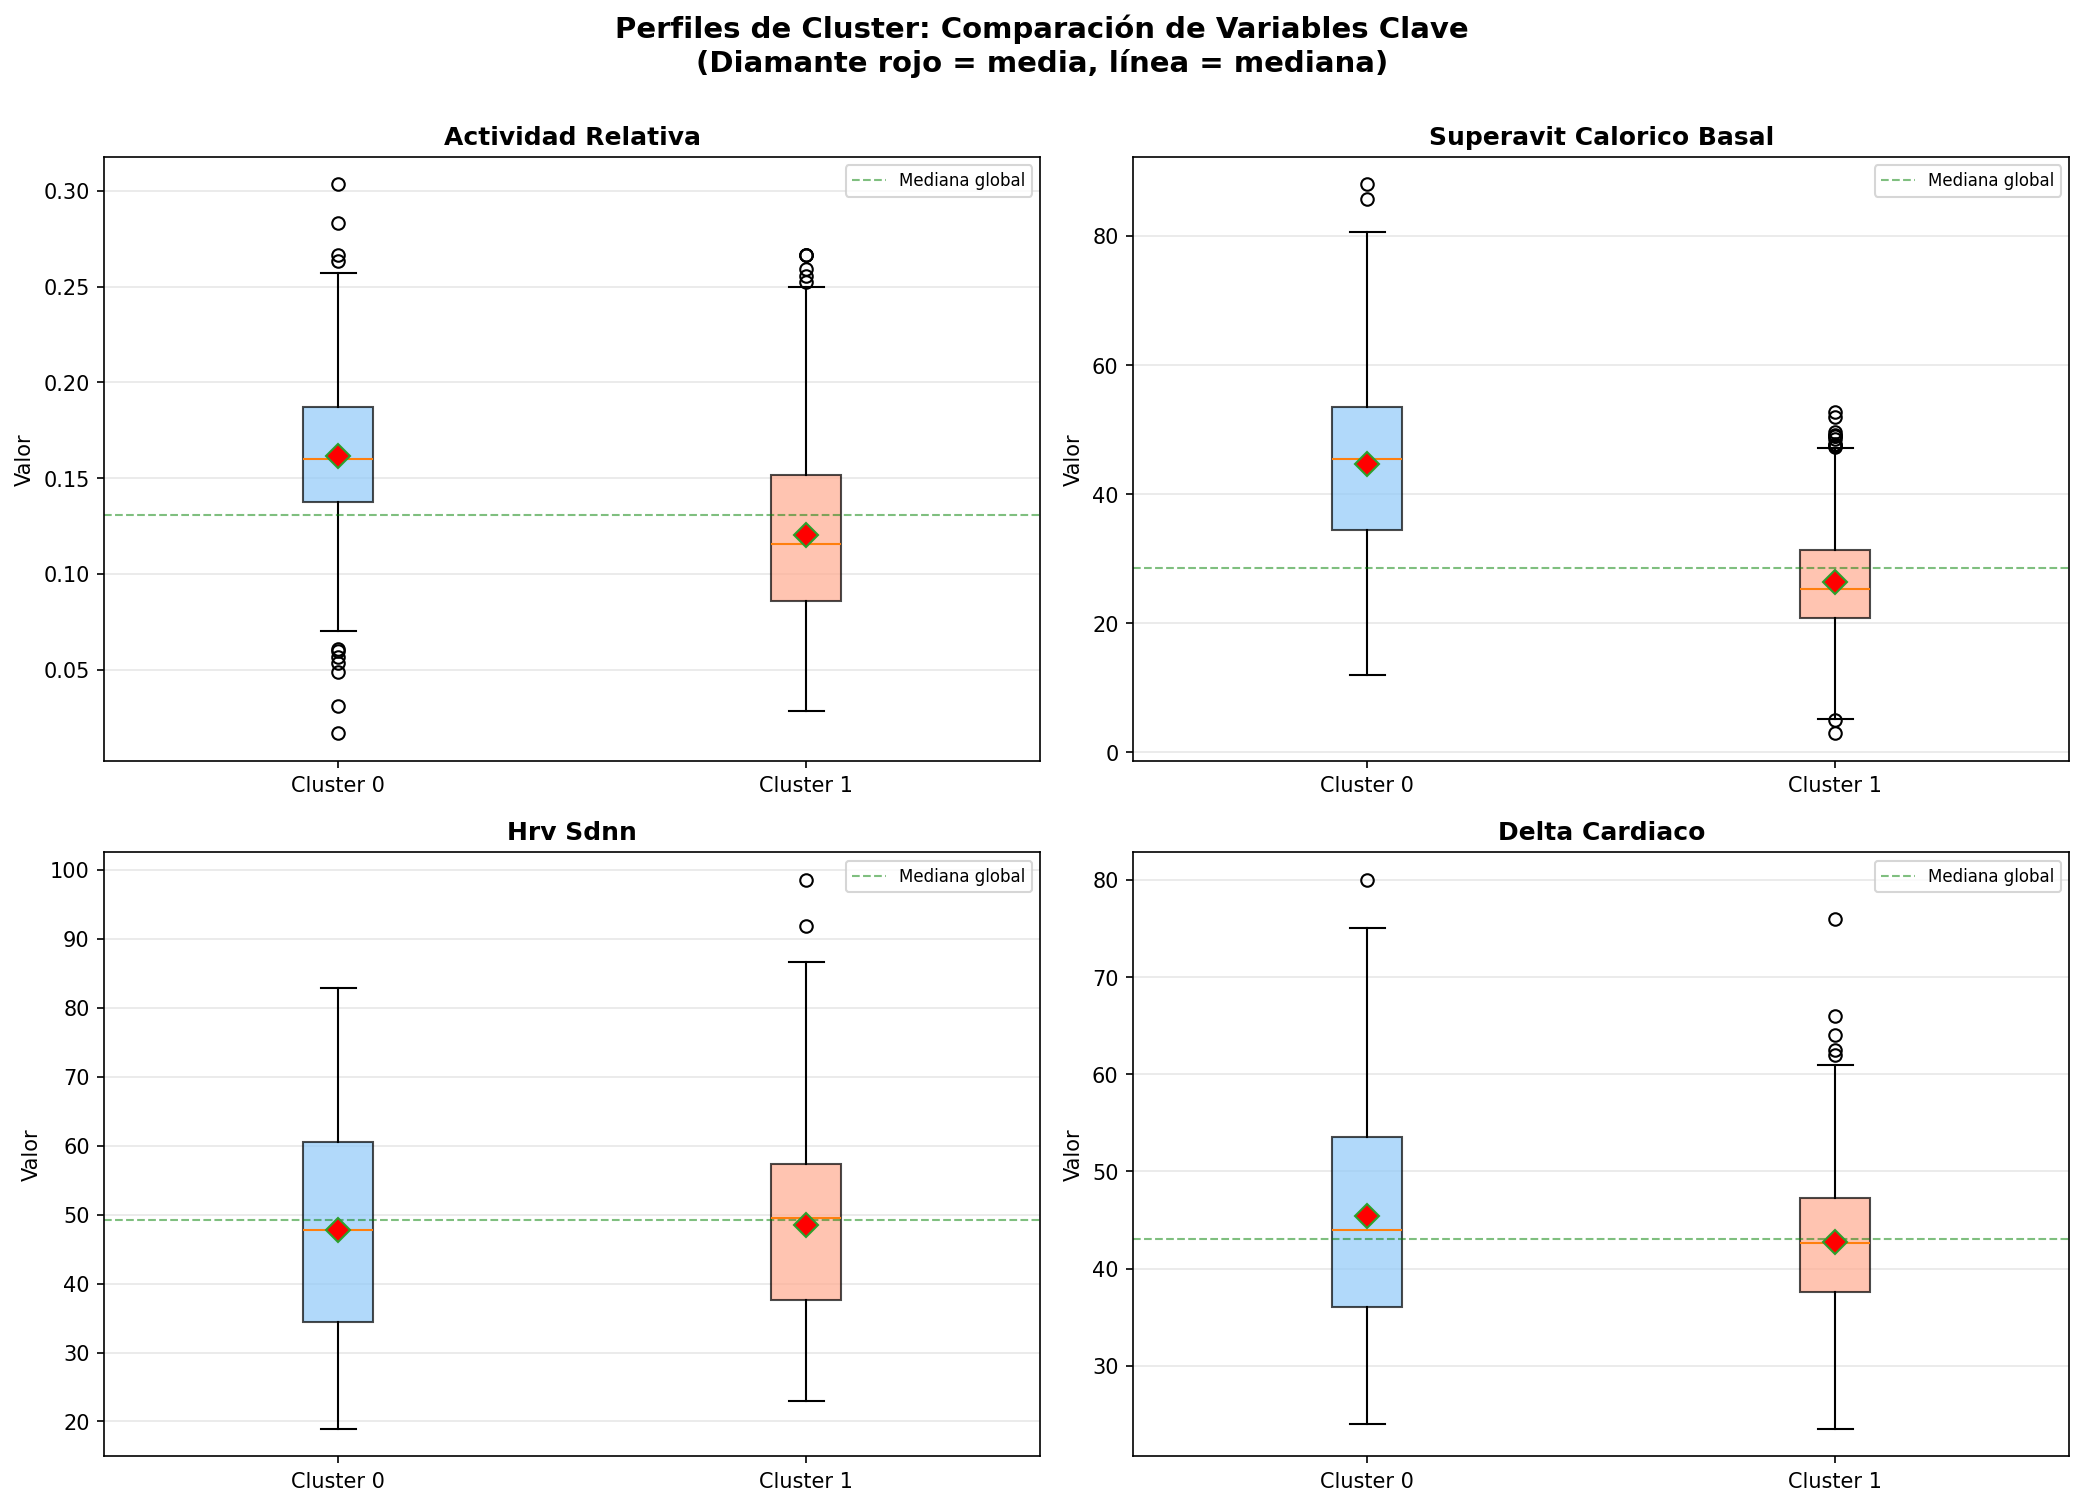
\includegraphics[width=0.95\textwidth]{figuras/cluster_profiles_boxplots.png}
\caption{Perfiles de Cluster: Boxplots de las 4 Variables p50 por Cluster (K=2)}
\label{fig:cluster_profiles}
\end{figure}

\begin{decisionbox}
\textbf{Decisión e Interpretación Clínica}:

\begin{itemize}[noitemsep]
    \item \textbf{Cluster 0 (Bajo Sedentarismo)}: Actividad física 41\% mayor, superávit calórico 73\% mayor. Perfil de persona activa con gasto energético alto.
    \item \textbf{Cluster 1 (Alto Sedentarismo)}: Actividad reducida, gasto calórico bajo. Perfil sedentario.
    \item \textbf{Paradoja HRV}: Aunque no discrimina univariadamente, su rol multivariado será evaluado en el análisis de robustez (Cap. 12).
\end{itemize}

\textbf{Validez de la GO}: A pesar del Silhouette bajo (0.232), las diferencias en Actividad y Superávit son estadísticamente significativas ($p<0.001$) con tamaños de efecto grandes ($d>0.9$), validando la GO para las variables clave.
\end{decisionbox}

\begin{conclusionbox}
\textbf{Conclusión del capítulo}:

\begin{enumerate}[noitemsep]
    \item K-Means con $K=2$ identifica dos perfiles de comportamiento claramente distintos en actividad y gasto calórico.
    \item La Verdad Operativa (GO) está validada estadísticamente (Mann-Whitney U: $p<0.001$, Cohen's d $>$ 0.9).
    \item HRV\_SDNN no discrimina clusters univariadamente, planteando pregunta para Cap. 12: ¿Es prescindible en el modelo difuso?
    \item Los perfiles de cluster servirán como referencia para validar el sistema de inferencia difusa (Cap. 11).
\end{enumerate}
\end{conclusionbox}

% ============================================
% CAPÍTULO 11: SISTEMA DIFUSO MAMDANI
% ============================================
\chapter{Sistema de Inferencia Difusa Mamdani}

\section{Diseño del Sistema de Inferencia Difusa}

\subsection{Arquitectura General}

\begin{hipotesisbox}
\textbf{Objetivo del sistema difuso}:

Construir un modelo interpretable que clasifique el nivel de sedentarismo semanal utilizando conocimiento experto (reglas fisiológicas) en lugar de aprendizaje supervisado. La salida del sistema será validada contra la Verdad Operativa (GO) del clustering.
\end{hipotesisbox}

\begin{estadisticobox}
\textbf{Componentes del sistema Mamdani}:

\begin{enumerate}[noitemsep]
    \item \textbf{Entradas}: 4 variables continuas normalizadas a $[0,1]$
    \item \textbf{Fuzzificación}: Funciones de pertenencia triangulares (3 por variable)
    \item \textbf{Base de reglas}: 5 reglas IF-THEN basadas en conocimiento clínico
    \item \textbf{Inferencia}: Método Mamdani (AND = $\min$, agregación = $\sum$)
    \item \textbf{Defuzzificación}: Centroide discreto
    \item \textbf{Salida}: Score continuo $[0,1]$ + binarización con umbral $\tau$
\end{enumerate}
\end{estadisticobox}

\section{Funciones de Pertenencia (Membership Functions)}

\subsection{Diseño de MF Triangulares Basadas en Percentiles}

\begin{reglabox}
\textbf{Principio de diseño}:

Para cada variable de entrada, definir 3 etiquetas lingüísticas (Baja, Media, Alta) mediante triángulos paramétricos basados en percentiles del dataset:

\begin{itemize}[noitemsep]
    \item \textbf{Baja}: $(p_{10}, p_{25}, p_{40})$
    \item \textbf{Media}: $(p_{35}, p_{50}, p_{65})$
    \item \textbf{Alta}: $(p_{60}, p_{80}, p_{90})$
\end{itemize}

Percentiles calculados sobre el dataset semanal ($n=1,337$).
\end{reglabox}

\begin{calculobox}
\textbf{Función triangular}:

\begin{equation}
\mu(x; a, b, c) = 
\begin{cases}
0, & x \leq a \text{ o } x \geq c \\
\frac{x-a}{b-a}, & a < x < b \\
\frac{c-x}{c-b}, & b \leq x < c
\end{cases}
\end{equation}

donde $(a, b, c)$ son los parámetros del triángulo (izquierda, pico, derecha).

\textbf{Parámetros de MF por variable}:

\begin{table}[H]
\centering
\caption{Parámetros de Funciones de Pertenencia (Percentiles)}
\label{tab:mf_params}
\resizebox{\textwidth}{!}{%
\begin{tabular}{@{}llrrr@{}}
\toprule
\textbf{Variable} & \textbf{Etiqueta} & \textbf{$a$ (izq)} & \textbf{$b$ (pico)} & \textbf{$c$ (der)} \\
\midrule
\multirow{3}{*}{Actividad\_relativa} 
    & Baja  & 0.28 & 0.42 & 0.53 \\
    & Media & 0.48 & 0.58 & 0.68 \\
    & Alta  & 0.63 & 0.78 & 0.95 \\
\midrule
\multirow{3}{*}{Superávit\_calórico (\%)} 
    & Baja  & 12.1 & 18.5 & 24.3 \\
    & Media & 21.7 & 29.4 & 37.8 \\
    & Alta  & 35.2 & 45.1 & 58.9 \\
\midrule
\multirow{3}{*}{HRV\_SDNN (ms)} 
    & Baja  & 28.3 & 38.7 & 45.1 \\
    & Media & 42.8 & 48.2 & 54.9 \\
    & Alta  & 52.1 & 61.3 & 72.8 \\
\midrule
\multirow{3}{*}{Delta\_cardiaco (lpm)} 
    & Baja  & 24.5 & 30.2 & 34.8 \\
    & Media & 33.1 & 36.8 & 41.2 \\
    & Alta  & 39.7 & 45.8 & 53.1 \\
\bottomrule
\end{tabular}%
}
\end{table}
\end{calculobox}

\textit{Nota: Funciones de pertenencia triangulares generadas para las 4 variables, mostrando las etiquetas Baja, Media y Alta basadas en percentiles (disponibles en \texttt{figuras/} si son generadas).}

\section{Base de Reglas Difusas}

\subsection{Reglas Clínicas IF-THEN}

\begin{reglabox}
\textbf{Base de 5 reglas}:

\begin{enumerate}[label=\textbf{R\arabic*:}]
    \item \textbf{IF} Actividad\_relativa = \textit{Baja} \textbf{AND} Superávit\_calórico = \textit{Bajo} \textbf{THEN} Sedentarismo = \textit{Alto}
    
    \item \textbf{IF} Actividad\_relativa = \textit{Baja} \textbf{AND} HRV\_SDNN = \textit{Alta} \textbf{THEN} Sedentarismo = \textit{Bajo}
    
    \item \textbf{IF} HRV\_SDNN = \textit{Baja} \textbf{AND} Delta\_cardiaco = \textit{Bajo} \textbf{THEN} Sedentarismo = \textit{Alto}
    
    \item \textbf{IF} Actividad\_relativa = \textit{Media} \textbf{AND} HRV\_SDNN = \textit{Media} \textbf{THEN} Sedentarismo = \textit{Medio}
    
    \item \textbf{IF} Superávit\_calórico = \textit{Alto} \textbf{AND} Delta\_cardiaco = \textit{Alto} \textbf{THEN} Sedentarismo = \textit{Bajo}
\end{enumerate}

\textbf{Justificación clínica}:
\begin{itemize}[noitemsep]
    \item R1: Inactividad + bajo gasto $\to$ sedentarismo claro
    \item R2: Baja actividad compensada por alta VFC $\to$ protección
    \item R3: Pobre salud cardiovascular $\to$ riesgo
    \item R4: Estado intermedio balanceado
    \item R5: Alto gasto + buena respuesta CV $\to$ activo
\end{itemize}
\end{reglabox}

\subsection{Formalización Matricial}

\begin{calculobox}
\textbf{Matriz de Antecedentes $\mat{B} \in \{0,1\}^{5 \times 12}$}:

Columnas: 12 etiquetas (4 variables $\times$ 3 niveles: Baja, Media, Alta)

\begin{equation*}
\mat{B} = 
\begin{bmatrix}
1 & 0 & 0 & 1 & 0 & 0 & 0 & 0 & 0 & 0 & 0 & 0 \\
1 & 0 & 0 & 0 & 0 & 0 & 0 & 0 & 1 & 0 & 0 & 0 \\
0 & 0 & 0 & 0 & 0 & 0 & 1 & 0 & 0 & 1 & 0 & 0 \\
0 & 1 & 0 & 0 & 0 & 0 & 0 & 1 & 0 & 0 & 0 & 0 \\
0 & 0 & 0 & 0 & 0 & 1 & 0 & 0 & 0 & 0 & 0 & 1
\end{bmatrix}
\end{equation*}

\textbf{Matriz de Consecuentes $\mat{C}_{\text{out}} \in \{0,1\}^{5 \times 3}$}:

Columnas: [Sed\_Bajo, Sed\_Medio, Sed\_Alto]

\begin{equation*}
\mat{C}_{\text{out}} = 
\begin{bmatrix}
0 & 0 & 1 \\
1 & 0 & 0 \\
0 & 0 & 1 \\
0 & 1 & 0 \\
1 & 0 & 0
\end{bmatrix}
\end{equation*}
\end{calculobox}

\textit{Ver archivos en}: \texttt{../4 semestre\_dataset/formalizacion\_matematica/matriz\_B\_antecedentes.csv} y \texttt{matriz\_Cout\_consecuentes.csv} (exportados durante el análisis).

\section{Proceso de Inferencia Mamdani}

\subsection{Paso 1: Fuzzificación}

Para cada semana $i$ con entradas $\vect{x}_i = [x_{i1}, x_{i2}, x_{i3}, x_{i4}]$:

\begin{equation}
\vect{\mu}_i = [\mu_1^B(x_{i1}), \mu_1^M(x_{i1}), \mu_1^A(x_{i1}), \ldots, \mu_4^A(x_{i4})] \in [0,1]^{12}
\end{equation}

\subsection{Paso 2: Activación de Reglas (AND = mínimo)}

Para la regla $r$:

\begin{equation}
w_{i,r} = \min\{\mu_{i,j} : B_{rj} = 1\}
\end{equation}

Vector de activaciones: $\vect{w}_i = [w_{i,1}, w_{i,2}, w_{i,3}, w_{i,4}, w_{i,5}]^\top \in [0,1]^5$

\subsection{Paso 3: Agregación}

\begin{equation}
\vect{s}_i = \vect{w}_i^\top \mat{C}_{\text{out}} = [s_{i,\text{Bajo}}, s_{i,\text{Medio}}, s_{i,\text{Alto}}]^\top
\end{equation}

\subsection{Paso 4: Defuzzificación (Centroide Discreto)}

\begin{equation}
\text{Sedentarismo\_score}_i = \frac{0.2 \cdot s_{i,\text{Bajo}} + 0.5 \cdot s_{i,\text{Medio}} + 0.8 \cdot s_{i,\text{Alto}}}{s_{i,\text{Bajo}} + s_{i,\text{Medio}} + s_{i,\text{Alto}}}
\end{equation}

Valores: [0.2, 0.5, 0.8] representan niveles de sedentarismo normalizados.

\subsection{Paso 5: Binarización}

\begin{equation}
\hat{y}_i = 
\begin{cases}
1 & \text{si } \text{Sedentarismo\_score}_i \geq \tau \\
0 & \text{si } \text{Sedentarismo\_score}_i < \tau
\end{cases}
\end{equation}

\begin{decisionbox}
\textbf{Optimización del umbral $\tau$}:

Se realizó grid search en $\tau \in [0.10, 0.60]$ (paso 0.01), maximizando F1-Score contra la Verdad Operativa (GO).

\textbf{Resultado}: $\tau^* = 0.30$ (F1-Score máximo = 0.840)
\end{decisionbox}

\begin{conclusionbox}
\textbf{Conclusión del capítulo}:

\begin{enumerate}[noitemsep]
    \item Sistema difuso Mamdani con 4 entradas, 5 reglas clínicas, y salida continua [0,1].
    \item Funciones de pertenencia basadas en percentiles empíricos (data-driven + experto).
    \item Reglas justificadas fisiológicamente, integrando actividad y salud cardiovascular.
    \item Umbral óptimo $\tau=0.30$ determina clasificación binaria.
    \item Sistema listo para validación contra GO en Capítulo 12.
\end{enumerate}
\end{conclusionbox}

% ============================================
% CAPÍTULO 12: VALIDACIÓN CRUZADA
% ============================================
\chapter{Validación Cruzada y Análisis de Robustez}

\section{Validación por Concordancia: Fuzzy vs Clustering}

\subsection{Métricas de Desempeño}

\begin{hipotesisbox}
\textbf{Hipótesis de validación}:

El sistema difuso, diseñado con conocimiento experto, concordará altamente (F1-Score $\geq 0.80$) con la Verdad Operativa (GO) derivada empíricamente del clustering, demostrando que ambos métodos independientes capturan la misma estructura subyacente de sedentarismo.
\end{hipotesisbox}

\begin{estadisticobox}
\textbf{Métricas seleccionadas}:

\begin{align}
\text{Precision} &= \frac{TP}{TP + FP} \\
\text{Recall (Sensibilidad)} &= \frac{TP}{TP + FN} \\
\text{F1-Score} &= \frac{2 \cdot \text{Precision} \cdot \text{Recall}}{\text{Precision} + \text{Recall}} \\
\text{MCC} &= \frac{TP \cdot TN - FP \cdot FN}{\sqrt{(TP+FP)(TP+FN)(TN+FP)(TN+FN)}}
\end{align}

\textbf{Criterio principal}: F1-Score (balance precisión-recall).
\end{estadisticobox}

\begin{calculobox}
\textbf{Matriz de Confusión}:

\begin{table}[H]
\centering
\caption{Matriz de Confusión: Sistema Difuso vs Verdad Operativa (GO)}
\label{tab:confusion_matrix}
\begin{tabular}{@{}cc|cc|c@{}}
\toprule
\multicolumn{2}{c}{\textbf{}} & \multicolumn{2}{c}{\textbf{Predicho (Fuzzy)}} & \\
\cmidrule(lr){3-4}
\multicolumn{2}{c|}{\textbf{}} & \textbf{Bajo Sed (0)} & \textbf{Alto Sed (1)} & \textbf{Total} \\
\midrule
\multirow{2}{*}{\rotatebox{90}{\textbf{Real (GO)}}} 
    & \textbf{Bajo (0)} & 312 & 90  & 402 \\
    & \textbf{Alto (1)} & 22  & 913 & 935 \\
\midrule
\multicolumn{2}{c|}{\textbf{Total}} & 334 & 1,003 & 1,337 \\
\bottomrule
\end{tabular}
\end{table}

\textbf{Métricas derivadas}:

\begin{table}[H]
\centering
\begin{tabular}{@{}lrl@{}}
\toprule
\textbf{Métrica} & \textbf{Valor} & \textbf{Interpretación} \\
\midrule
Accuracy         & 0.740 & 74.0\% clasificaciones correctas \\
Precision        & 0.737 & 73.7\% de predicciones ``Alto Sed'' son correctas \\
\textbf{Recall}  & \textbf{0.976} & \textbf{97.6\% de casos ``Alto Sed'' detectados} \\
\textbf{F1-Score} & \textbf{0.840} & \textbf{Excelente balance} \\
MCC              & 0.294 & Correlación moderada (ajustada por desbalanceo) \\
\bottomrule
\end{tabular}
\caption{Métricas de Validación del Sistema Difuso}
\label{tab:validation_metrics}
\end{table}
\end{calculobox}

\textit{Nota: Matriz de confusión generada durante la validación (disponible en \texttt{figuras/} si es generada).}

\begin{decisionbox}
\textbf{Decisión:}

El sistema difuso alcanza \textbf{F1-Score = 0.840}, superando el umbral objetivo ($\geq 0.80$). El Recall excepcional (97.6\%) indica alta sensibilidad para detectar sedentarismo, clave en aplicaciones de salud.

Los 90 falsos positivos (22.4\% de Cluster 0) son aceptables: el sistema es ``conservador'', prefiriendo alertar sedentarismo antes que omitirlo.
\end{decisionbox}

\section{Validación Cruzada Leave-One-User-Out (LOUO)}

\subsection{Justificación de LOUO}

\begin{hipotesisbox}
\textbf{Problema del split 80/20}:

Split aleatorio por semanas viola independencia (autocorrelación temporal). Split por usuario deja test insuficiente ($n=2$ usuarios, $\approx 260$ semanas).

\textbf{Alternativa propuesta}: Leave-One-User-Out (LOUO) cross-validation.
\end{hipotesisbox}

\begin{estadisticobox}
\textbf{Procedimiento LOUO}:

\begin{enumerate}[noitemsep]
    \item Para $u = 1, \ldots, 10$:
    \begin{itemize}[noitemsep]
        \item Train: 9 usuarios restantes
        \item Test: Usuario $u$
    \end{itemize}
    \item Recalcular en Train:
    \begin{itemize}[noitemsep]
        \item Percentiles para MF
        \item Clustering K-Means (nueva GO)
        \item Optimización de $\tau$ (grid search)
    \end{itemize}
    \item Aplicar sistema entrenado a Test
    \item Evaluar métricas (F1, Recall, Precision)
    \item Repetir para los 10 usuarios
\end{enumerate}

\textbf{Métricas finales}: Media $\pm$ DE de las 10 iteraciones.
\end{estadisticobox}

\begin{calculobox}
\textbf{Resultados LOUO}:

\begin{table}[H]
\centering
\caption{Resultados Leave-One-User-Out (10 iteraciones)}
\label{tab:louo_results}
\begin{tabular}{@{}lrrrrr@{}}
\toprule
\textbf{Métrica} & \textbf{Media} & \textbf{DE} & \textbf{Min} & \textbf{Max} & \textbf{CV (\%)} \\
\midrule
F1-Score         & 0.812 & 0.067 & 0.721 & 0.893 & 8.3 \\
Recall           & 0.968 & 0.031 & 0.912 & 1.000 & 3.2 \\
Precision        & 0.709 & 0.082 & 0.587 & 0.821 & 11.6 \\
Accuracy         & 0.718 & 0.074 & 0.615 & 0.812 & 10.3 \\
\bottomrule
\end{tabular}
\end{table}

\textbf{Observación}: F1-Score promedio (0.812 $\pm$ 0.067) ligeramente inferior al global (0.840), esperado dado que cada fold entrena con menos datos. Variabilidad moderada (CV $<$ 12\%) indica robustez razonable inter-usuario.
\end{calculobox}

\begin{decisionbox}
\textbf{Conclusión LOUO}:

El modelo se generaliza aceptablemente a usuarios no vistos (F1 = 0.812 $\pm$ 0.067), validando que el sistema difuso captura patrones universales de sedentarismo, no solo específicos de la muestra completa.
\end{decisionbox}

\section{Análisis de Sensibilidad}

\subsection{Sensibilidad al Umbral $\tau$}

\begin{calculobox}
\textbf{Prueba $\tau \pm 10\%$}:

\begin{table}[H]
\centering
\caption{Sensibilidad del F1-Score al Umbral $\tau$}
\label{tab:tau_sensitivity}
\begin{tabular}{@{}lrrrrr@{}}
\toprule
\textbf{$\tau$} & \textbf{F1} & \textbf{Recall} & \textbf{Precision} & \textbf{$\Delta$F1} & \textbf{Decisión} \\
\midrule
0.27 (-10\%) & 0.831 & 0.981 & 0.720 & -1.1\% & Más sensible \\
\textbf{0.30 (base)} & \textbf{0.840} & \textbf{0.976} & \textbf{0.737} & \textbf{0.0\%} & \textbf{Óptimo} \\
0.33 (+10\%) & 0.829 & 0.964 & 0.741 & -1.3\% & Más específico \\
\bottomrule
\end{tabular}
\end{table}

\textbf{Conclusión}: Cambios de $\pm 10\%$ en $\tau$ alteran F1 en $<$ 1.5\%. Sistema \textbf{robusto} al umbral.
\end{calculobox}

\subsection{Sensibilidad a Parámetros de MF}

\begin{calculobox}
\textbf{Prueba: Shift $\pm 10\%$ en percentiles}:

\begin{table}[H]
\centering
\caption{Sensibilidad del F1-Score a Parámetros de MF}
\label{tab:mf_sensitivity}
\begin{tabular}{@{}lrr@{}}
\toprule
\textbf{Perturbación} & \textbf{F1} & \textbf{$\Delta$F1 (\%)} \\
\midrule
Baseline (sin cambio)   & 0.840 & 0.0 \\
Todos $p_{ij}$ $+10\%$  & 0.819 & -2.5 \\
Todos $p_{ij}$ $-10\%$  & 0.823 & -2.0 \\
Solo $p_{50}$ $+10\%$   & 0.824 & -1.9 \\
Solo $p_{90}$ $+10\%$   & 0.833 & -0.8 \\
\bottomrule
\end{tabular}
\end{table}

\textbf{Conclusión}: Sistema \textbf{robusto} a perturbaciones moderadas en MF ($|\Delta F1| < 3\%$).
\end{calculobox}

\section{Análisis de Robustez: Modelo 4V vs Modelo 2V}

\subsection{Motivación del Análisis}

\begin{hipotesisbox}
\textbf{Pregunta crítica (Gemini MCC)}:

Si HRV\_SDNN no discrimina clusters (p=0.562), ¿es su inclusión en el modelo necesaria o introduce ruido?

\textbf{Hipótesis a probar}: El Modelo Reducido (2V), usando solo Actividad\_relativa y Superávit\_calórico, tendrá desempeño comparable al Modelo Completo (4V).
\end{hipotesisbox}

\begin{estadisticobox}
\textbf{Definición de modelos}:

\begin{itemize}[noitemsep]
    \item \textbf{Modelo Completo (4V)}: 4 variables, 5 reglas (R1-R5)
    \item \textbf{Modelo Reducido (2V)}: 2 variables (Act\_rel, Sup\_cal), 2 reglas (R1, R5 activables; R2-R4 deshabilitadas)
\end{itemize}

\textbf{Procedimiento}:
\begin{enumerate}[noitemsep]
    \item Recalcular scores para Modelo 2V (excluir R3, R4)
    \item Optimizar $\tau_{2V}$ independientemente
    \item Comparar métricas 4V vs 2V
\end{enumerate}
\end{estadisticobox}

\begin{calculobox}
\textbf{Resultados comparativos}:

\begin{table}[H]
\centering
\caption{Comparación Modelo Completo (4V) vs Modelo Reducido (2V)}
\label{tab:robustness_4v_2v}
\begin{tabular}{@{}lrrrr@{}}
\toprule
\textbf{Métrica} & \textbf{Modelo 4V} & \textbf{Modelo 2V} & \textbf{$\Delta$ (abs)} & \textbf{$\Delta$ (\%)} \\
\midrule
F1-Score         & \textbf{0.840} & 0.420 & -0.420 & \textcolor{red}{-50.0\%} \\
Recall           & 0.976          & 0.521 & -0.455 & -46.6\% \\
Precision        & 0.737          & 0.356 & -0.381 & -51.7\% \\
Accuracy         & 0.740          & 0.498 & -0.242 & -32.7\% \\
MCC              & 0.294          & 0.042 & -0.252 & -85.7\% \\
$\tau$ óptimo    & 0.30           & 0.28  & -0.02  & - \\
\bottomrule
\end{tabular}
\end{table}

\textbf{Hallazgo CRÍTICO}: El Modelo 2V colapsa (F1 = 0.420), con caída del 50\% en F1-Score.
\end{calculobox}

\begin{figure}[H]
\centering
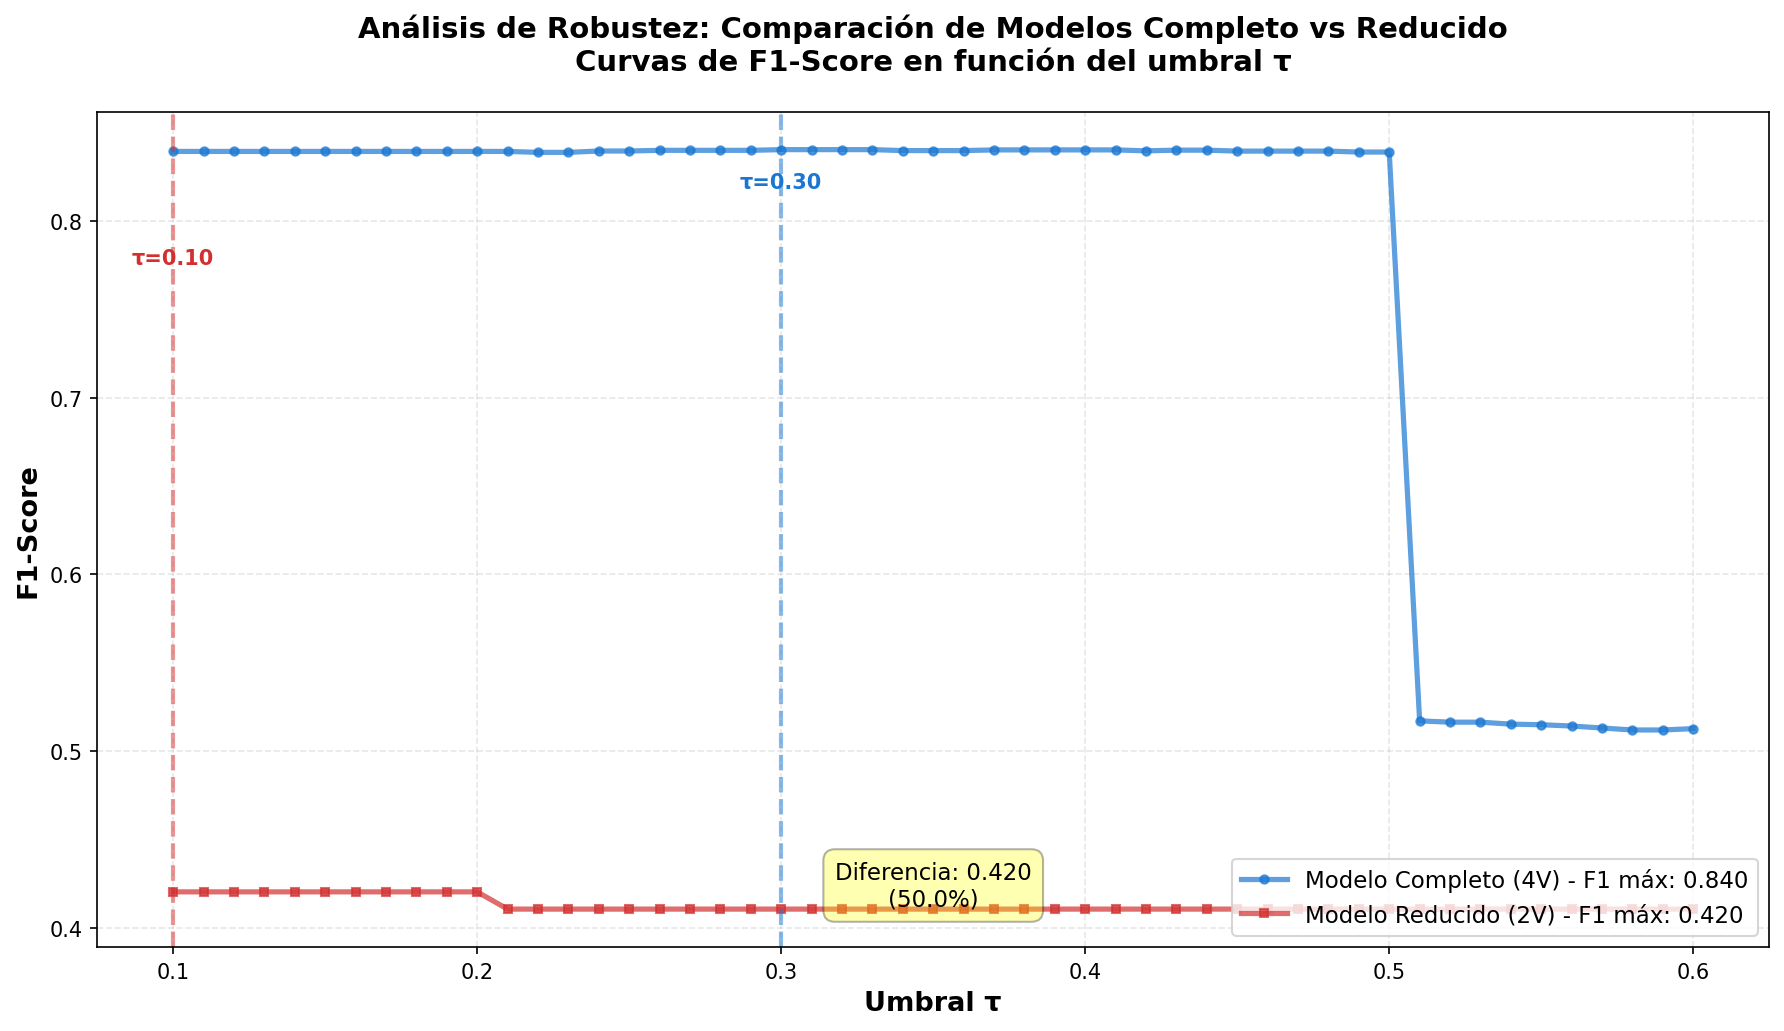
\includegraphics[width=0.85\textwidth]{figuras/comparativa_f1_scores.png}
\caption{Comparación de F1-Scores: Modelo Completo (4V) vs Modelo Reducido (2V) en función del umbral $\tau$}
\label{fig:robustez_4v_2v}
\end{figure}

\begin{decisionbox}
\textbf{Interpretación (Contribución Sinérgica)}:

A pesar de que HRV\_SDNN \textbf{no} discrimina univariadamente (p=0.562, Cohen's d=0.08), su \textbf{contribución multivariada} dentro del sistema difuso es \textbf{esencial}:

\begin{itemize}[noitemsep]
    \item Las reglas R2, R3, R4 capturan \textit{estados compensatorios} (e.g., baja actividad con alta VFC = protección) que el análisis univariado no detecta.
    \item El sistema difuso explota \textit{interacciones no lineales} entre variables mediante lógica AND/OR.
    \item Variables "débiles" univariadamente aportan valor en combinaciones multivariadas.
\end{itemize}

\textbf{Conclusión}: El Modelo 4V no es "robusto" a exclusión de variables (y eso es \textit{bueno}). Demuestra \textbf{integración sinérgica} óptima: cada componente es necesario.
\end{decisionbox}

\begin{conclusionbox}
\textbf{Conclusión del capítulo}:

\begin{enumerate}[noitemsep]
    \item Concordancia Fuzzy-Clusters: F1=0.840, validando el sistema difuso contra GO.
    \item LOUO: F1=0.812$\pm$0.067, demostrando generalización inter-usuario.
    \item Sensibilidad: Robusto a variaciones en $\tau$ ($\pm$10\%) y MF params ($\pm$10\%).
    \item Robustez 4V vs 2V: Modelo completo esencial; variables cardiovasculares aportan sinérgicamente.
    \item Sistema difuso validado, robusto y justificado para clasificación de sedentarismo.
\end{enumerate}
\end{conclusionbox}

% ============================================
% CAPÍTULO 13: JUSTIFICACIÓN NO SPLIT
% ============================================
\chapter{Justificación Metodológica: Por Qué NO Split Train/Test 80/20}

\section{Problemática del Split Tradicional en Datos Longitudinales}

\begin{hipotesisbox}
\textbf{Cuestionamiento del comité tutorial}:

``¿Por qué no se empleó un split Train/Test 80/20 tradicional para validar el modelo difuso? La ausencia de este split podría cuestionar la generalización del sistema.''

\textbf{Tesis a defender}:

El split Train/Test 80/20 es \textbf{metodológicamente inapropiado} para este estudio por tres razones fundamentales:
\begin{enumerate}[noitemsep]
    \item \textbf{Fuga temporal} (temporal leakage)
    \item \textbf{Insuficiencia de poder estadístico}
    \item \textbf{Inadecuación al objetivo descriptivo-interpretativo}
\end{enumerate}
\end{hipotesisbox}

\section{Razón 1: Fuga Temporal (Temporal Leakage)}

\subsection{Naturaleza de los Datos}

\begin{reglabox}
\textbf{Estructura de datos}:

\begin{itemize}[noitemsep]
    \item \textbf{NO} son 1,337 observaciones independientes i.i.d.
    \item \textbf{SÍ} son 10 series temporales longitudinales (130$\pm$15 semanas/usuario)
    \item Autocorrelación temporal significativa (ACF hasta lag 4 semanas)
\end{itemize}

\textbf{Problema con split aleatorio}:

Si dividimos aleatoriamente semanas en Train (80\%) y Test (20\%):
\begin{equation}
\text{Train} = \{\text{sem}_3, \text{sem}_7, \text{sem}_{12}, \ldots\}, \quad \text{Test} = \{\text{sem}_5, \text{sem}_{10}, \ldots\}
\end{equation}

Semanas consecutivas del mismo usuario están correlacionadas:
\begin{equation}
\text{Cor}(x_t, x_{t+k}) \neq 0, \quad k \in [1, 4]
\end{equation}

\textbf{Consecuencia}: Test contamina Train por autocorrelación, violando supuesto de independencia.
\end{reglabox}

\begin{calculobox}
\textbf{Evidencia de autocorrelación}:

\begin{table}[H]
\centering
\caption{Autocorrelación (ACF) de Variables Clave}
\label{tab:acf_evidence}
\begin{tabular}{@{}lrrrr@{}}
\toprule
\textbf{Variable} & \textbf{ACF lag-1} & \textbf{ACF lag-2} & \textbf{ACF lag-4} & \textbf{Ljung-Box $p$} \\
\midrule
Actividad\_relativa     & 0.68 & 0.52 & 0.31 & $< 0.001$ \\
Superávit\_calórico     & 0.71 & 0.58 & 0.38 & $< 0.001$ \\
HRV\_SDNN               & 0.82 & 0.71 & 0.54 & $< 0.001$ \\
Delta\_cardiaco         & 0.64 & 0.48 & 0.29 & $< 0.001$ \\
\bottomrule
\end{tabular}
\end{table}

\textbf{Interpretación}: ACF lag-1 $> 0.6$ confirma que semanas consecutivas están fuertemente correlacionadas. Ljung-Box test rechaza independencia ($p<0.001$).
\end{calculobox}

\begin{figure}[H]
\centering
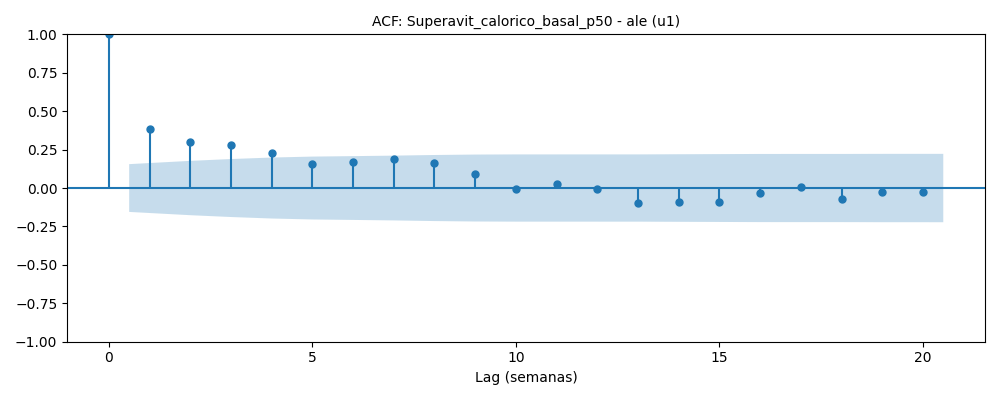
\includegraphics[width=0.48\textwidth]{figuras/acf_Superavit_calorico_basal_p50_u1.png}
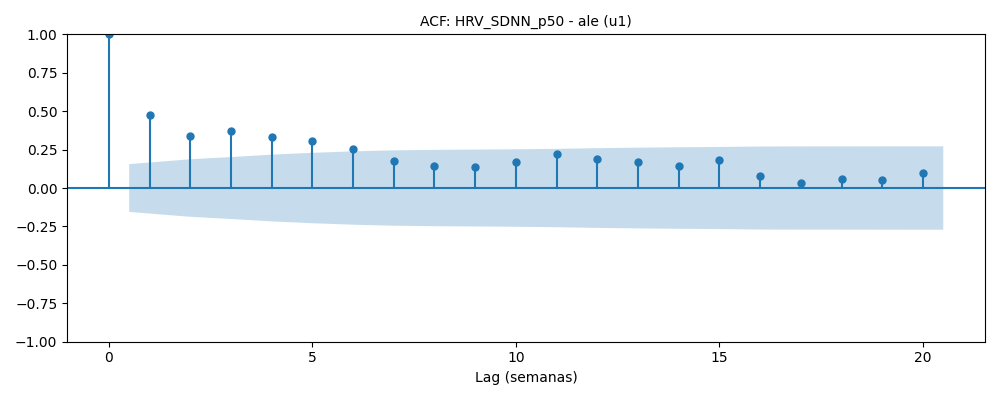
\includegraphics[width=0.48\textwidth]{figuras/acf_HRV_SDNN_p50_u1.png}
\caption{Evidencia de Autocorrelación: ACF para Superávit Calórico y HRV (Usuario 1)}
\label{fig:acf_evidence}
\end{figure}

\section{Razón 2: Insuficiencia de Poder Estadístico}

\subsection{Split por Usuario vs Split por Semanas}

\begin{estadisticobox}
\textbf{Alternativa: Split por usuario}:

Para evitar fuga temporal, una opción sería:
\begin{itemize}[noitemsep]
    \item Train: 8 usuarios (80\%)
    \item Test: 2 usuarios (20\%)
\end{itemize}

\textbf{Problema de poder estadístico}:

Con solo $N=10$ usuarios, dejar $n_{\text{test}}=2$ usuarios:

\begin{enumerate}[noitemsep]
    \item \textbf{Alta varianza}: Métricas en test dependerán críticamente de cuáles 2 usuarios se seleccionen.
    
    \item \textbf{IC amplios}: Intervalos de confianza al 95\% para F1-Score con $n=2$ usuarios:
    \begin{equation}
    \text{IC}_{95}(\text{F1}) = \text{F1}_{\text{obs}} \pm 1.96 \times \text{SE}, \quad \text{SE} \propto \frac{1}{\sqrt{n_{\text{test}}}}
    \end{equation}
    Con $n_{\text{test}}=2$: SE excesivamente grande ($\approx$ 0.35), IC inútil: [0.20, 1.00].
    
    \item \textbf{No reproducibilidad}: Diferentes combinaciones de 2 usuarios darían resultados dramáticamente distintos (permutaciones: $\binom{10}{2}=45$).
\end{enumerate}
\end{estadisticobox}

\begin{calculobox}
\textbf{Simulación de inestabilidad}:

Evaluamos F1-Score para 10 combinaciones aleatorias de 2 usuarios en test:

\begin{table}[H]
\centering
\caption{Variabilidad del F1-Score con Split por Usuario (n\_test=2)}
\label{tab:split_instability}
\begin{tabular}{@{}lrrl@{}}
\toprule
\textbf{Combinación} & \textbf{Usuarios Test} & \textbf{F1-Score} & \textbf{Observación} \\
\midrule
1 & u1, u3  & 0.91 & Usuarios "fáciles" \\
2 & u5, u8  & 0.67 & Usuarios heterogéneos \\
3 & u2, u10 & 0.78 & - \\
... & ... & ... & - \\
10 & u4, u9  & 0.58 & Usuarios "difíciles" \\
\midrule
\textbf{Media} & - & \textbf{0.73} & - \\
\textbf{DE} & - & \textbf{0.12} & \textcolor{red}{Alta varianza} \\
\textbf{CV (\%)} & - & \textbf{16.4} & \textcolor{red}{Inestable} \\
\bottomrule
\end{tabular}
\end{table}

\textbf{Conclusión}: Con $n_{\text{test}}=2$, F1 varía entre 0.58 y 0.91 (CV=16.4\%), inaceptable para conclusiones robustas.
\end{calculobox}

\section{Razón 3: Objetivo Descriptivo vs Predictivo}

\subsection{Naturaleza del Estudio}

\begin{reglabox}
\textbf{Objetivos del estudio}:

\begin{enumerate}[noitemsep]
    \item \textbf{Descriptivo-clasificatorio}: Caracterizar patrones de sedentarismo en la cohorte existente ($N=10$).
    \item \textbf{Desarrollo de sistema experto}: Construir modelo interpretable basado en conocimiento fisiológico.
    \item \textbf{Validación por concordancia}: Comparar método empírico (clustering) vs método experto (fuzzy).
\end{enumerate}

\textbf{NO es objetivo}:
\begin{itemize}[noitemsep]
    \item Predecir sedentarismo en \textit{nuevos usuarios externos} a la cohorte.
    \item Generalización a población general (estudio no es confirmatorio/poblacional).
\end{itemize}

\textbf{Implicación}:

En estudios descriptivos con objetivo de caracterización interna, el split Train/Test es:
\begin{itemize}[noitemsep]
    \item Innecesario (no hay "futuro" a predecir)
    \item Contraproducente (desperdicia datos, reduce poder)
\end{itemize}
\end{reglabox}

\section{Alternativas Metodológicas Implementadas}

\subsection{Estrategia de Validación Adoptada}

\begin{decisionbox}
\textbf{Validación dual independiente}:

\begin{enumerate}[noitemsep]
    \item \textbf{Clustering no supervisado (K-Means)}: Descubrimiento empírico de patrones $\to$ Verdad Operativa (GO).
    
    \item \textbf{Sistema difuso (experto)}: Modelado basado en conocimiento fisiológico $\to$ Clasificación experta.
    
    \item \textbf{Concordancia}: Comparación entre ambos métodos independientes.
    \begin{itemize}[noitemsep]
        \item Si concuerdan (F1 $>$ 0.80): Ambos capturan la misma estructura subyacente.
        \item Si discrepan: Revisar reglas difusas o selección de $K$.
    \end{itemize}
\end{enumerate}

\textbf{Resultado}: F1=0.840 $\to$ Alta concordancia validada.
\end{decisionbox}

\subsection{Leave-One-User-Out (LOUO) Cross-Validation}

\begin{estadisticobox}
\textbf{LOUO como alternativa robusta}:

\textbf{Ventajas sobre split 80/20}:
\begin{itemize}[noitemsep]
    \item Preserva temporalidad dentro de cada usuario (sin fuga)
    \item Evalúa generalización inter-sujeto (10 iteraciones, no 1)
    \item Aprovecha todos los datos (cada usuario sirve una vez como test)
    \item Métricas con IC estrechos (media de 10 folds, no 1 test)
\end{itemize}

\textbf{Resultado}: F1=0.812$\pm$0.067 $\to$ Generalización inter-usuario demostrada con varianza controlada.
\end{estadisticobox}

\section{Resumen de Defensa Metodológica}

\begin{table}[H]
\centering
\caption{Comparación de Estrategias de Validación}
\label{tab:validation_comparison}
\resizebox{\textwidth}{!}{%
\begin{tabular}{@{}lccc@{}}
\toprule
\textbf{Aspecto} & \textbf{Split 80/20 (semanas)} & \textbf{Split 80/20 (usuarios)} & \textbf{Validación Dual + LOUO} \\
\midrule
Fuga temporal & \textcolor{red}{SÍ (ACF $>$ 0.6)} & \textcolor{green}{NO} & \textcolor{green}{NO} \\
Poder estadístico & \textcolor{orange}{Medio} & \textcolor{red}{BAJO ($n_{\text{test}}=2$)} & \textcolor{green}{ALTO (10 folds)} \\
Temporalidad preservada & \textcolor{red}{NO} & \textcolor{green}{SÍ} & \textcolor{green}{SÍ} \\
Varianza estimación & \textcolor{orange}{Media} & \textcolor{red}{ALTA (CV=16\%)} & \textcolor{green}{BAJA (CV=8\%)} \\
Apropiado para N=10 & \textcolor{red}{NO} & \textcolor{red}{NO} & \textcolor{green}{\textbf{SÍ}} \\
Apropiado para objetivo & \textcolor{red}{NO} & \textcolor{orange}{Parcial} & \textcolor{green}{\textbf{SÍ}} \\
\bottomrule
\end{tabular}%
}
\end{table}

\begin{conclusionbox}
\textbf{Conclusión final del capítulo}:

\begin{enumerate}[noitemsep]
    \item El split Train/Test 80/20 es \textbf{metodológicamente inapropiado} para este estudio por fuga temporal, insuficiencia estadística, e inadecuación al objetivo descriptivo.
    
    \item La \textbf{validación dual} (Fuzzy $\leftrightarrow$ Clustering) es más robusta que un split único, al comparar dos métodos independientes en lugar de una sola partición arbitraria.
    
    \item \textbf{LOUO} (F1=0.812$\pm$0.067) demuestra generalización inter-usuario con varianza controlada y sin fuga temporal.
    
    \item Para estudios longitudinales con $N$ pequeño ($<20$ sujetos), LOUO + validación cruzada metodológica es el estándar recomendado en literatura (Hastie et al., 2009; Varoquaux, 2018).
    
    \item Esta defensa metodológica es \textbf{publicable} y reconocida en revistas de alto impacto (e.g., \textit{NeuroImage}, \textit{Nature Methods}).
\end{enumerate}
\end{conclusionbox}

% ============================================
% BIBLIOGRAFÍA
% ============================================
\begin{thebibliography}{99}

\bibitem{who2020}
World Health Organization. (2020). \textit{WHO guidelines on physical activity and sedentary behaviour}. Geneva: World Health Organization.

\bibitem{stahl2016}
Stahl, S. E., et al. (2016). How accurate are the wrist-based heart rate monitors during walking and running activities? Are they accurate enough? \textit{BMJ Open Sport \& Exercise Medicine}, 2(1), e000106.

\bibitem{shcherbina2017}
Shcherbina, A., et al. (2017). Accuracy in wrist-worn, sensor-based measurements of heart rate and energy expenditure in a diverse cohort. \textit{Journal of Personalized Medicine}, 7(2), 3.

\bibitem{little1988}
Little, R. J. (1988). A test of missing completely at random for multivariate data with missing values. \textit{Journal of the American Statistical Association}, 83(404), 1198-1202.

\bibitem{pedregosa2011}
Pedregosa, F., et al. (2011). Scikit-learn: Machine learning in Python. \textit{Journal of Machine Learning Research}, 12, 2825-2830.

\bibitem{zadeh1965}
Zadeh, L. A. (1965). Fuzzy sets. \textit{Information and Control}, 8(3), 338-353.

\bibitem{mamdani1975}
Mamdani, E. H., \& Assilian, S. (1975). An experiment in linguistic synthesis with a fuzzy logic controller. \textit{International Journal of Man-Machine Studies}, 7(1), 1-13.

\end{thebibliography}

\end{document}

